\documentclass{beamer}
\usepackage[utf8]{inputenc}
\usepackage[portuguese]{babel}
\usepackage{amsmath}
\usepackage{subfigure}
\usepackage{booktabs}

\usetheme{metropolis}           % Use metropolis theme

\newtheorem{mydefinition}{Definição}

\newcommand{\foreignword}[1]{\textit{#1}}
\newcommand{\toolname}[1]{\textit{#1}}
\newcommand{\fieldR}{\mathbb{R}}
\newcommand{\powerset}{\mathcal{P}}
\newcommand{\probability}{\mathbb{P}}
\newcommand{\expectation}{\mathbb{E}}
\newcommand{\algname}[1]{\texttt{#1}}
\newcommand{\langname}[1]{\texttt{#1}}
\newcommand{\varname}[1]{\texttt{#1}}
\newcommand{\floor}[1]{\lfloor #1 \rfloor}
\newcommand{\ceil}[1]{\lceil #1 \rceil}
\newcommand{\mathsc}[1]{{\normalfont\textsc{#1}}}
\newcommand{\forest}{\mathcal{F}}
\newcommand{\pfsnode}[1]{\mathbf #1}
\newcommand{\species}[1]{\textit{#1}}
\newcommand{\gender}[1]{\textit{#1}}

\graphicspath{ {img/} }

\title{Projeto de Algoritmos Baseados em Florestas de Posets para o
Problema de Otimização U-curve}
\date{Novembro de 2017}
\author{Gustavo Estrela}
\institute{Instituto de Matemática e Estatística \\ 
           Centro de Toxinas, Resposta-imune e Sinalização Celular (CeTICS) \\
           Laboratório Especial de Ciclo Celular, Instituto Butantan}
\begin{document}
  \maketitle
    
  \section{O problema U-curve}

\begin{frame}{Modelos computacionais}
  Modelos computacionais são criados para simular sistemas complexos. \\
  \pause
  \begin{center}
  %\alert{ 
  $
  \begin{aligned}
    \text{entrada} &\longrightarrow& \text{sistema} &\longrightarrow& \text{saída} \\
    \pause
    \text{entrada} &\longrightarrow& \text{modelo} &\longrightarrow& \sim\text{saída} \\
  \end{aligned}
  $
  %}
  \end{center}
\end{frame} 

\begin{frame}{Exemplo de modelo computacional}
  \begin{figure}
    \centering
    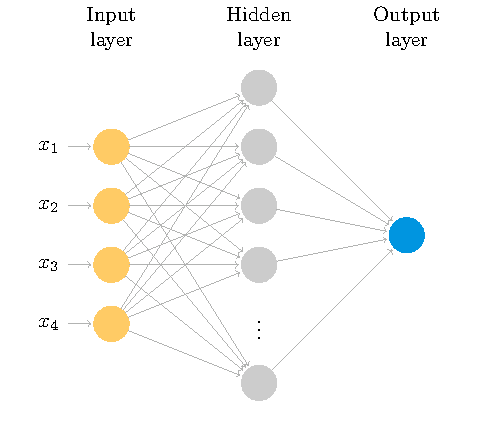
\includegraphics[clip=true]{neuralnet/neuralnet.pdf}
  \end{figure}
\end{frame}

\begin{frame}{O problema de seleção de características}
  A seleção de características é uma etapa da seleção de modelos. Ela
  deve escolher quais são as melhores características para se considerar
  no modelo.
  \pause
  \begin{mydefinition}
    Dado um conjunto $S$ de características e uma função 
    de custo $c$, ache o subconjunto de 
    $X \in \powerset(S)$ tal que $c (X)$ é mínimo.
  \end{mydefinition}
\end{frame}


\begin{frame}{O problema de seleção de características}
  Podemos representar um conjunto $X$ de características por um vetor
  de bits que chamamos de \alert{vetor característico}. \\
  %\pause
  %Assuma que o conjunto $S$ tem uma ordem $S = \langle s_1, s_2, ..., s_n \rangle$.
  %Então, se o conjunto $X$ possui a i-ésima característica de $S$, então
  %o i-ésimo bit do vetor característico deve estar ligado.
  \pause
  \vspace{1em}
  Por exemplo, se $S = \{s_1, s_2, s_3\}$ e $X = \{s_1, s_3\}$
  então o vetor característico de $X$ é $101$.
\end{frame}

\begin{frame}{O espaço de busca}
  Os algoritmos estudados neste trabalho representam o espaço de busca
  com o reticulado Booleano $(\powerset(S), \subseteq)$.
  \begin{figure}
    \centering
    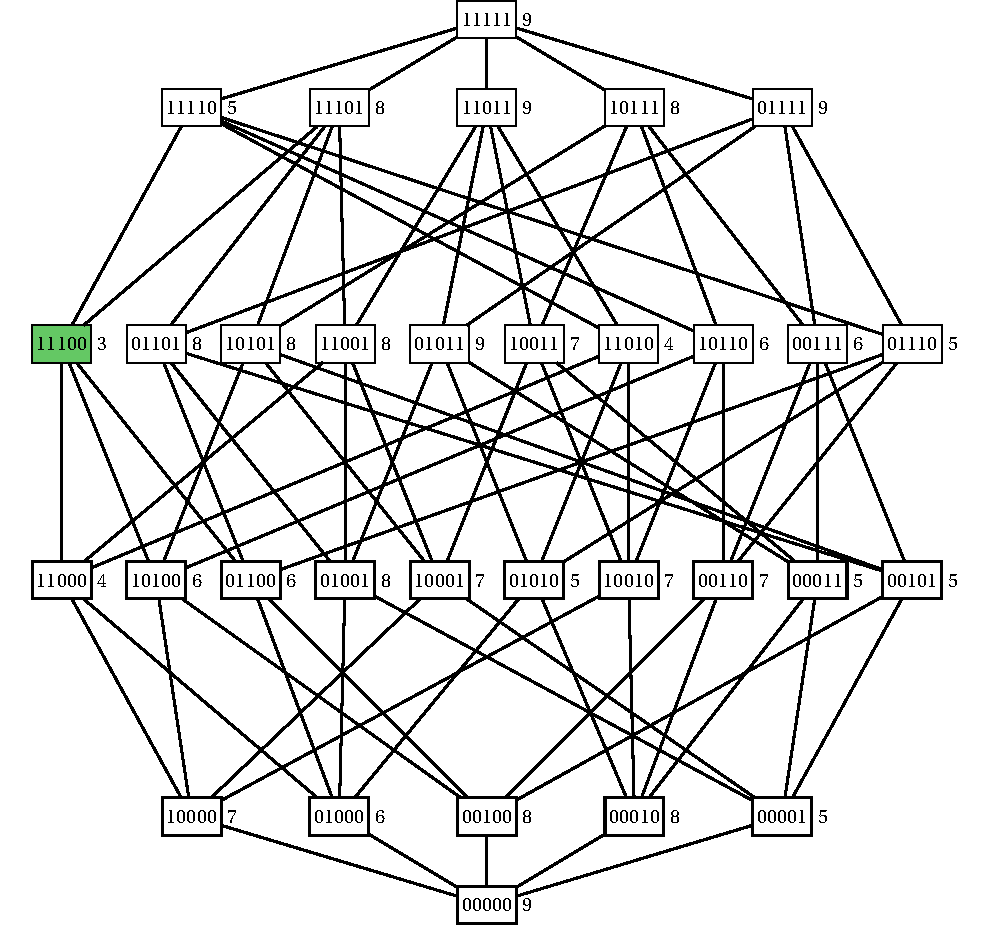
\includegraphics[clip=true, width=.6\textwidth]{lattice/Boolean_lattice.pdf}
  \end{figure}
\end{frame}

\begin{frame}{O espaço de busca}
  Chamamos de \alert{cadeia} uma sequência de conjuntos adjacentes 
  $X_1, X_2, \dots, X_n$ tal que $X_1 \subseteq X_2 \subseteq \dots \subseteq X_n$. 
  \pause
  \begin{figure}
    \centering
    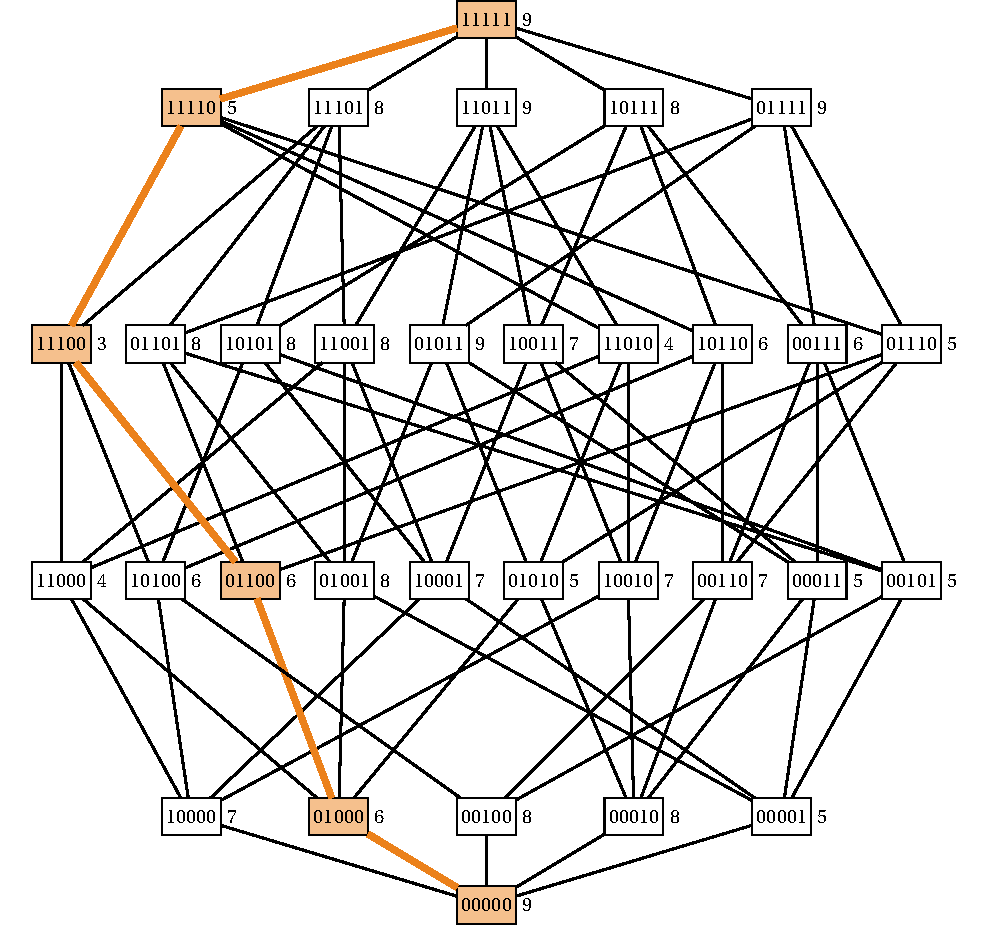
\includegraphics[clip=true, width=.6\textwidth]{lattice/chain.pdf}
  \end{figure}
\end{frame}

\begin{frame}{A função de custo}
  A função de custo $c$ deve refletir a qualidade de um conjunto de 
  características $X$ a ser usado no modelo.\\
  \pause
  \vspace{1em}
  Nestas funções, um fenômeno conhecido em aprendizado de máquina aparece.
  A função descreve curvas em U nas cadeias do reticulado.
  \begin{figure}[ht]
    \centering
    \begin{tabular}{c c}
    \subfigure {\scalebox{.4}{
        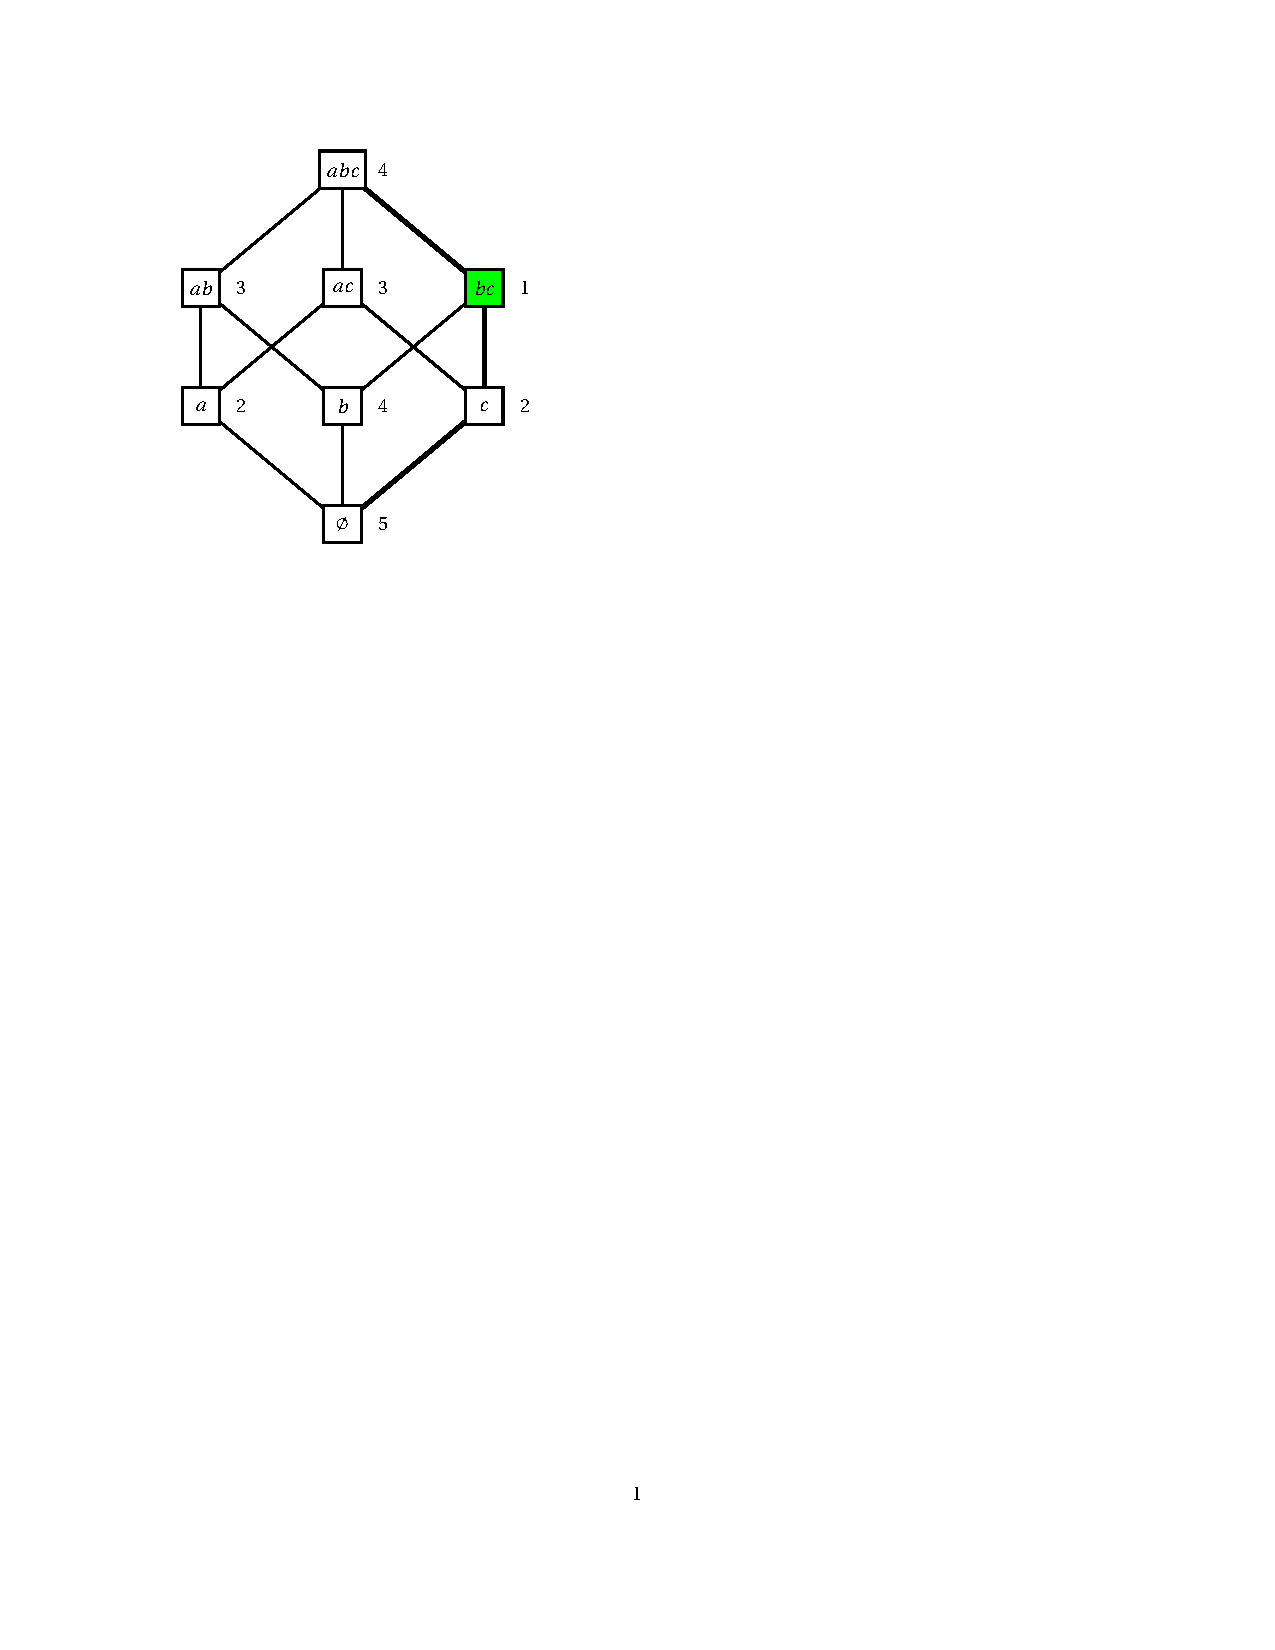
\includegraphics[clip=true, trim={3cm 18cm 13cm 2cm}]{intro/example_lattice_3.pdf}}
    \label{fig:intro:lattice} }
    & 
    \subfigure {\scalebox{.15}{
        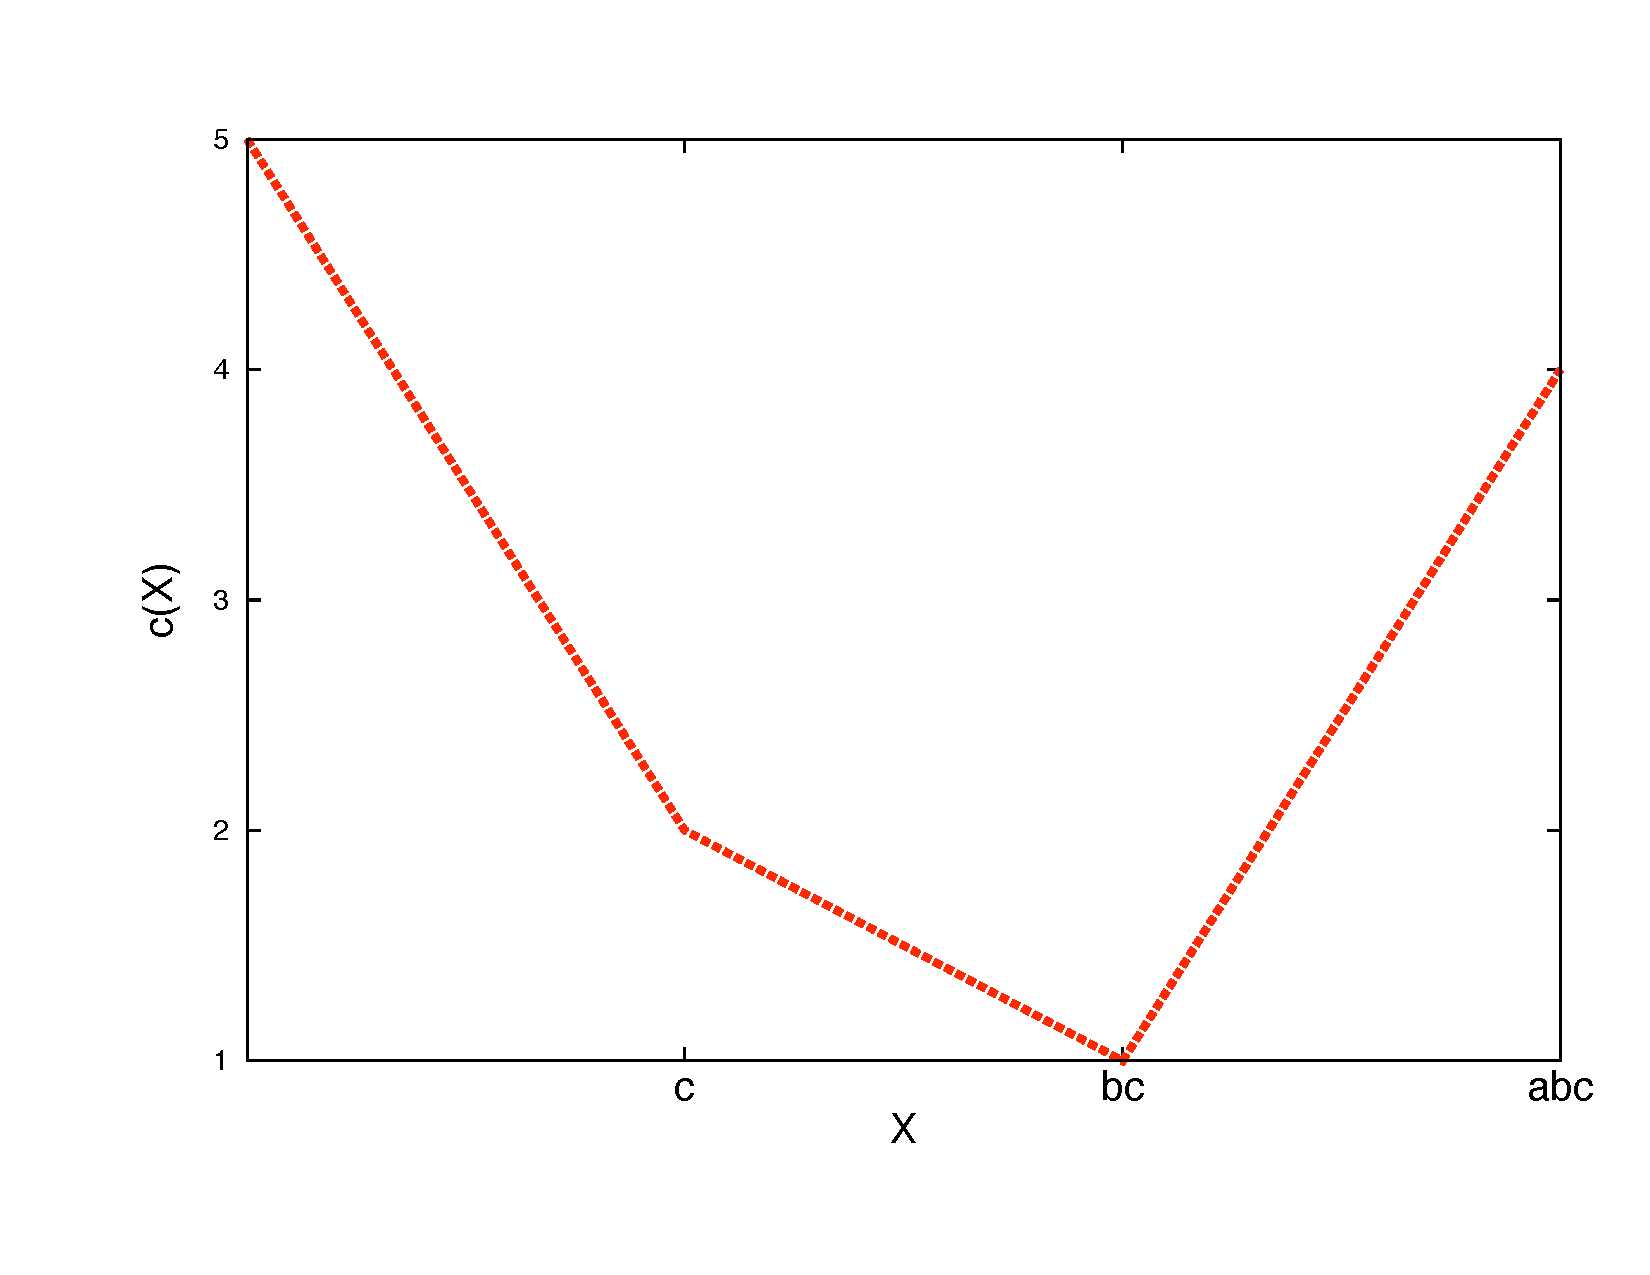
\includegraphics[clip=true, trim={1cm 0cm 1cm 2cm}]{intro/example_lattice_chain_3.pdf}}
    \label{fig:intro:chain} }
    \end{tabular}
\end{figure}
\end{frame}

\begin{frame}{Funções decomponíveis em curvas U}
\begin{mydefinition}\label{fund_concepts:ushape}
Uma função de custo $c$ é dita {\bf \em decomponível em curvas U} se
para toda cadeia maximal $X_1, ..., X_l$, $c(X_j) \leq max \{c (X_i),
c (X_k)\}$ sempre que $X_i \subseteq X_j \subseteq X_k$, $i, j, k \in 
\{1, ..., l\}$.
\end{mydefinition}
\end{frame}


\begin{frame}{O problema U-curve}
\begin{mydefinition}[Problema U-Curve]
Dados um conjunto finito e não-vazio $S$ e uma função de custo $c$ 
decomponível em curvas U, encontrar um subconjunto $X \in \powerset (S)$ 
tal que $c(X)$ é mínimo.
\end{mydefinition}
\end{frame}

\section{Algoritmos baseados em florestas}
\begin{frame}{O algoritmo \algname{U-Curve-Branch-and-Bound}}
O algoritmo \algname{U-Curve-Branch-and-Bound} (\algname{UBB}) organiza
o espaço de busca em uma árvore.
\begin{figure}[!ht]
  \centering 
  \begin{tabular}{c c}
    \subfigure {\scalebox{0.3}{
     \includegraphics[clip=true]{pfs/ubb/full_lattice.pdf}}
     \label{fig:ubb:full} }
    & 
    \subfigure {\scalebox{.3}{
    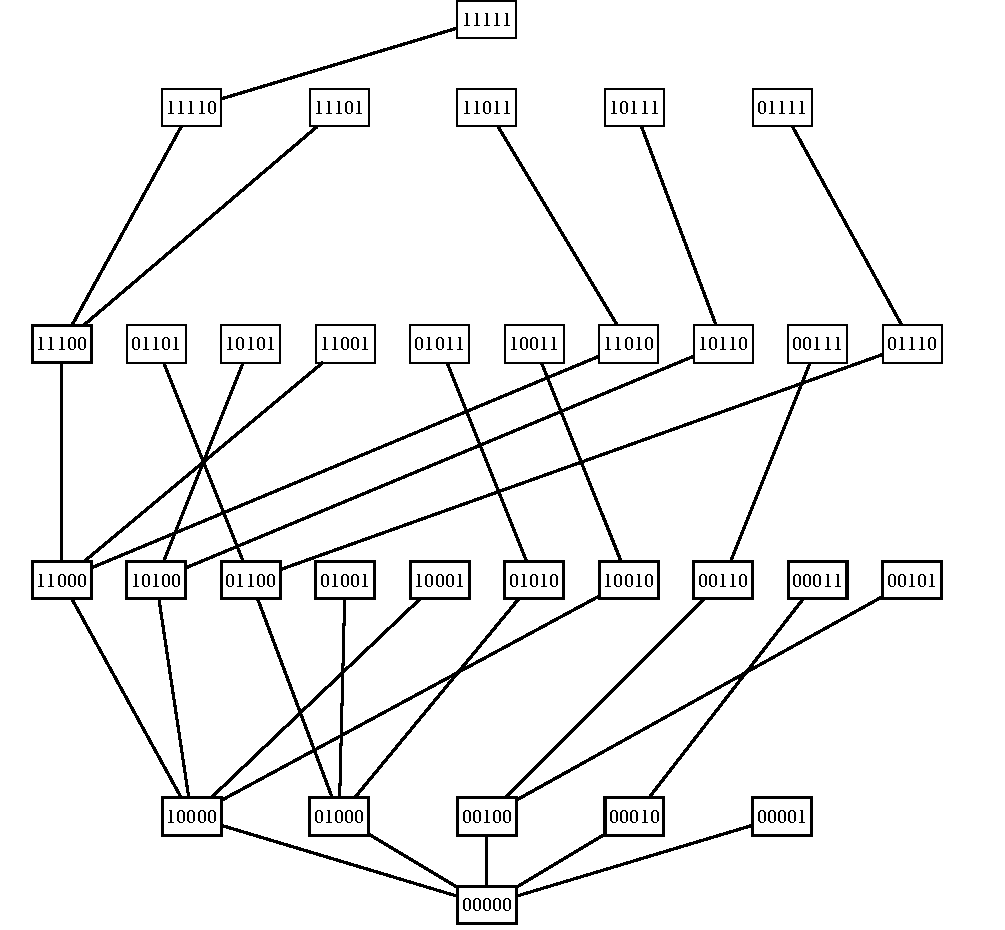
\includegraphics[clip=true]{pfs/ubb/ubb_tree.pdf}}
    \label{fig:ubb:tree} }
  \end{tabular}
\end{figure}  
\end{frame}

\begin{frame}{O algoritmo \algname{U-Curve-Branch-and-Bound}}
Este algoritmo busca o mínimo global ramificando na árvore como em uma
busca em profundidade e faz podas sempre que o custo aumenta.
\begin{figure}[!ht]
  \centering 
  \begin{tabular}{c c}
    \subfigure {\scalebox{0.3}{
     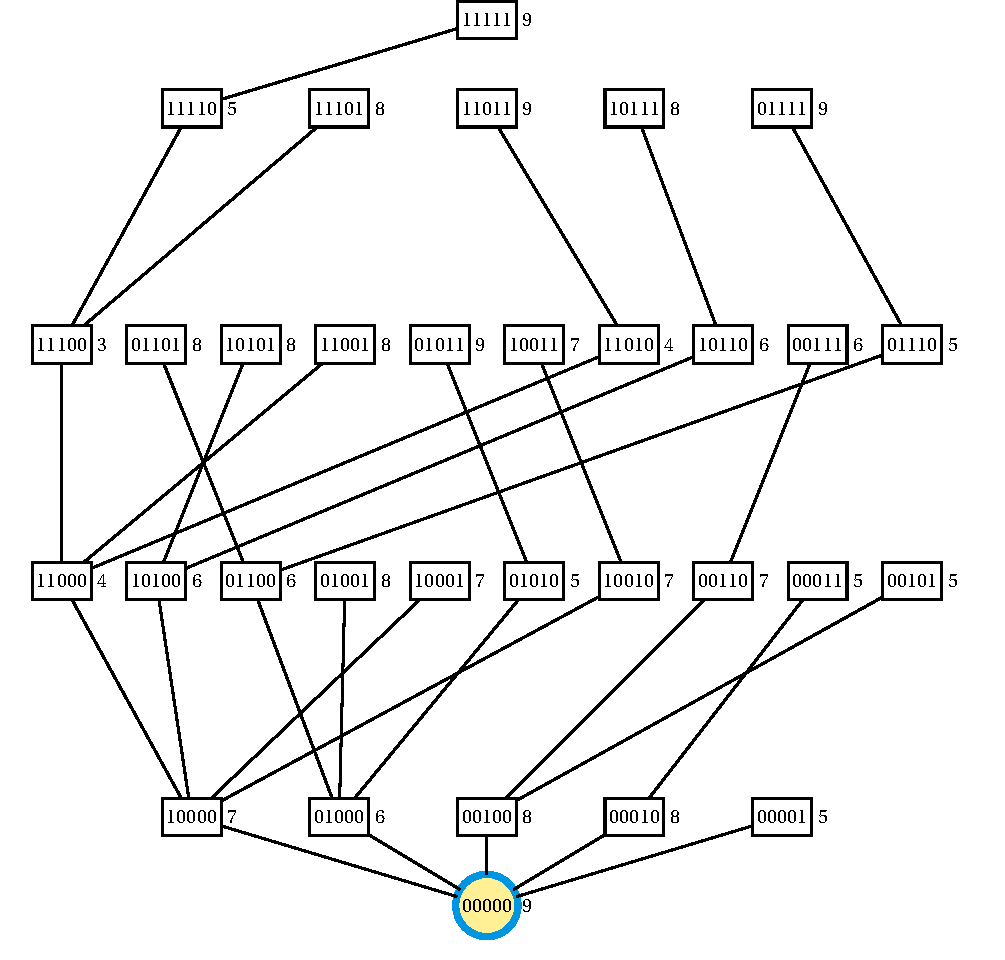
\includegraphics[clip=true]{pfs/ubb_run/b.pdf}}
     \label{fig:ubb:full} }
    & 
    \pause
    \subfigure {\scalebox{.3}{
    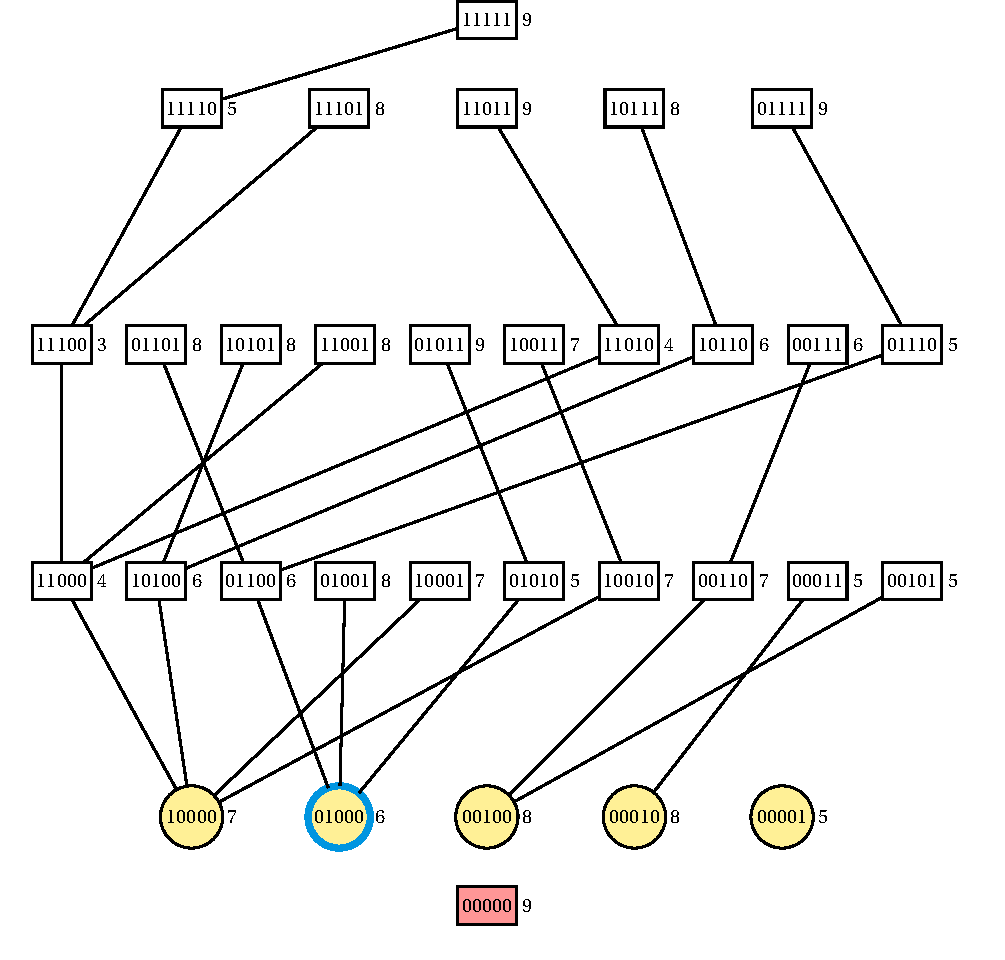
\includegraphics[clip=true]{pfs/ubb_run/c.pdf}}
    \label{fig:ubb:tree} }
  \end{tabular}
\end{figure}  
\end{frame}

\begin{frame}{O algoritmo \algname{U-Curve-Branch-and-Bound}}
\begin{figure}[!ht]
  \centering 
  \begin{tabular}{c c}
    \subfigure {\scalebox{0.3}{
     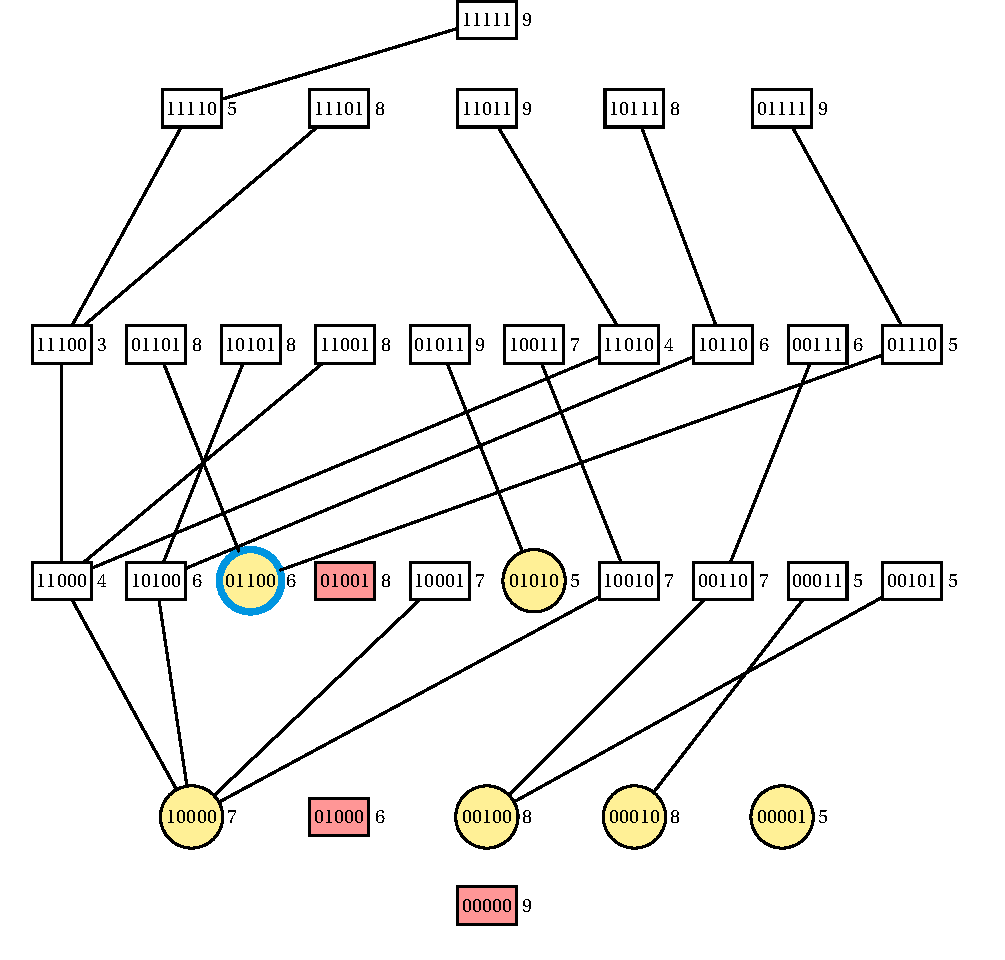
\includegraphics[clip=true]{pfs/ubb_run/d.pdf}}
     \label{fig:ubb:full} }
    \pause
    & 
    \subfigure {\scalebox{.3}{
    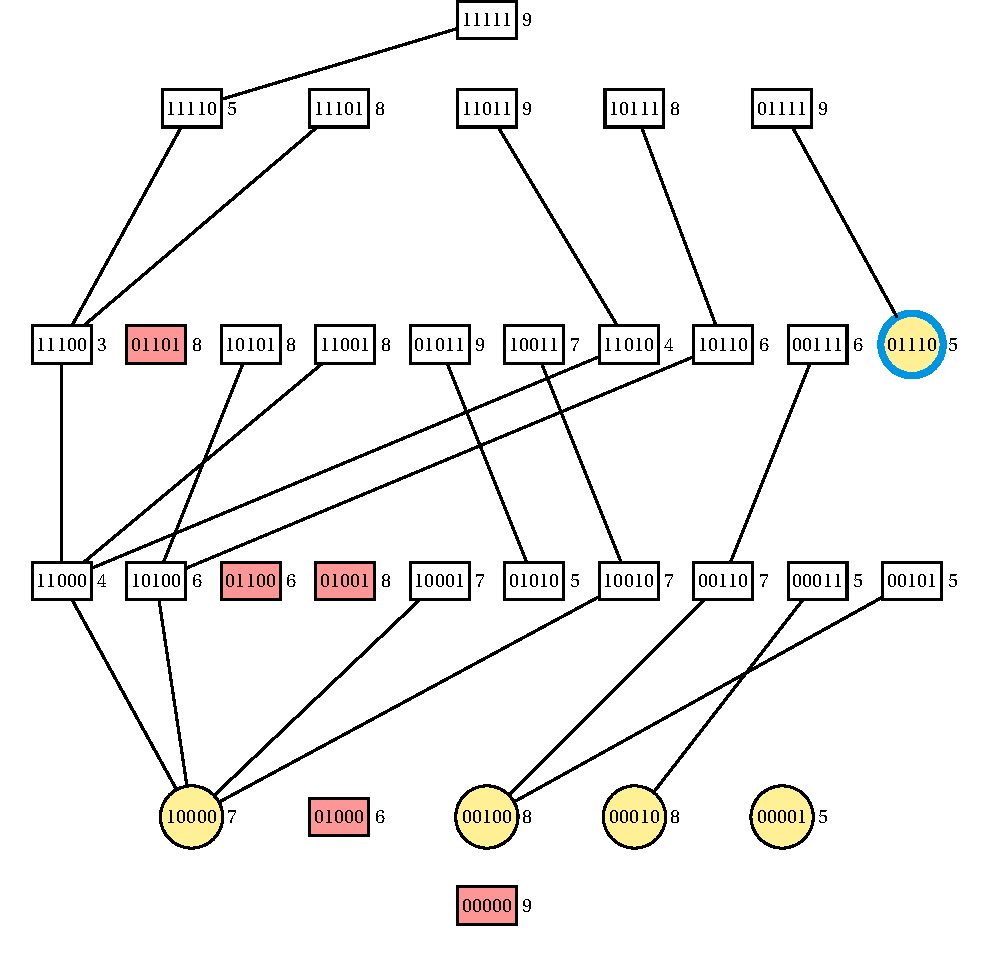
\includegraphics[clip=true]{pfs/ubb_run/e.pdf}}
    \label{fig:ubb:tree} }
  \end{tabular}
\end{figure}  
\pause
Note que se a condição de poda nunca é verdadeira, então o espaço
de busca inteiro é percorrido.
\end{frame}

\begin{frame}{O algoritmo \algname{Poset-Forest-Search}}
  Solução: percorrer o espaço de busca em duas direções.
  \pause
  %\vspace{1em}
  
  O algoritmo \algname{Poset-Fores-Search} (\algname{PFS}) pode fazer
  isso porque decompõe o espaço em duas árvores.
  \begin{figure}[!ht]
  \centering 
  \begin{tabular}{c c}
    \subfigure {\scalebox{0.28}{
     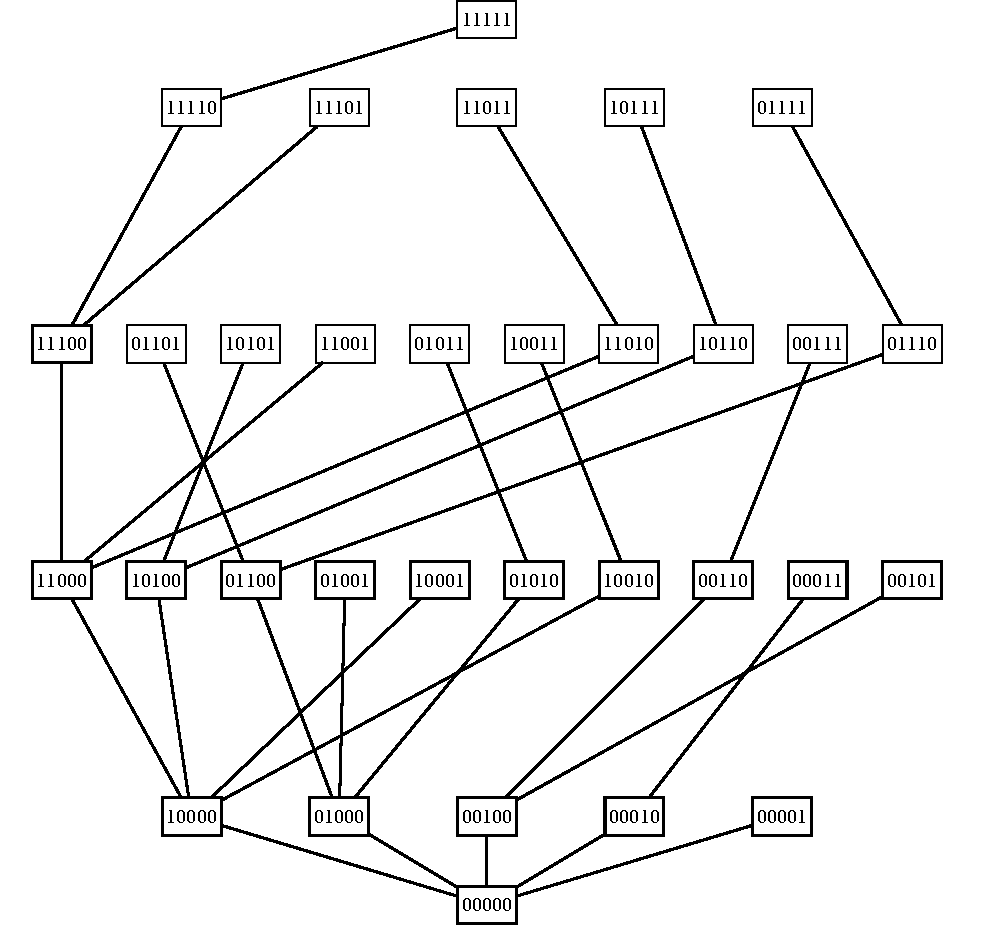
\includegraphics[clip=true]{pfs/pfs/lower_tree.pdf}}
     \label{fig:ubb:full} }
    \pause
    & 
    \subfigure {\scalebox{.28}{
    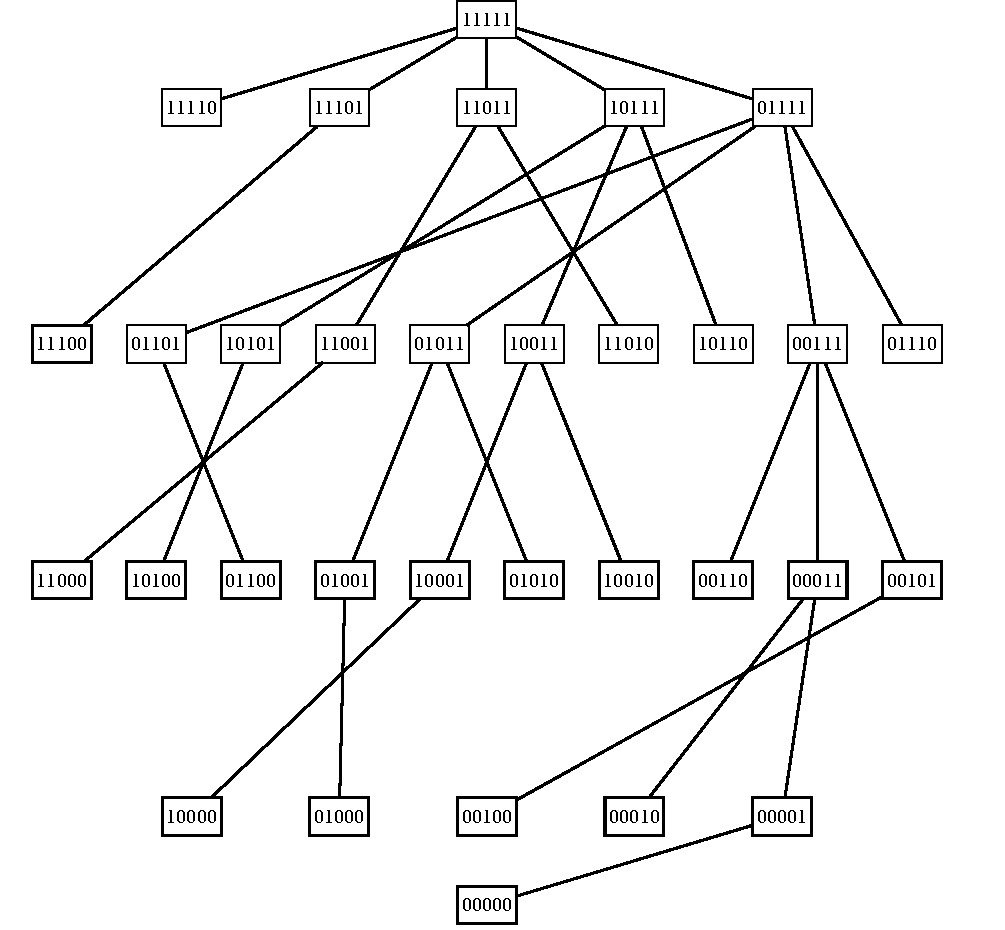
\includegraphics[clip=true]{pfs/pfs/upper_tree.pdf}}
    \label{fig:ubb:tree} }
  \end{tabular}
  \end{figure}  
\end{frame}

\begin{frame}{O algoritmo \algname{Poset-Forest-Search}}
  Problema: agora é necessário manter as duas árvores equivalentes,
  ou seja, representando o mesmo espaço de busca.
  \begin{figure}[!ht]
  \centering 
  \begin{tabular}{c c}
    \subfigure {\scalebox{0.28}{
     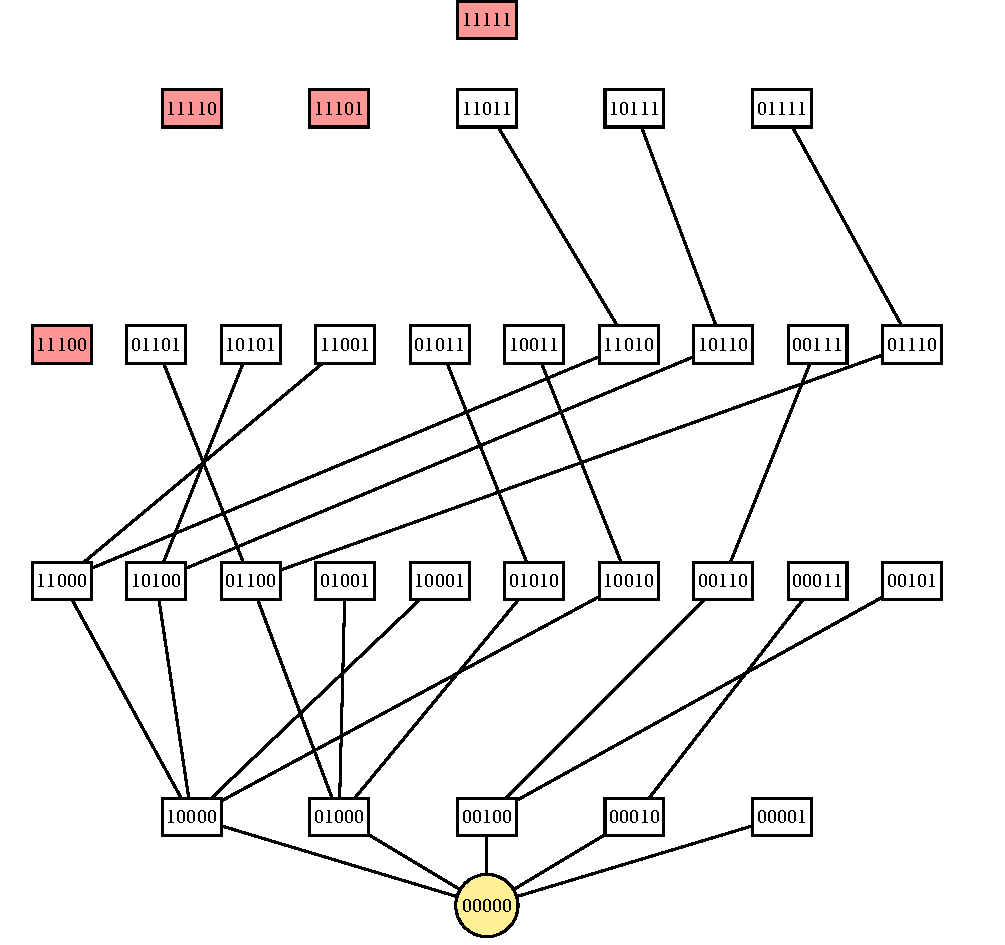
\includegraphics[clip=true]{pfs/pfs/forest/lower_tree.pdf}}
     \label{fig:ubb:full} }
    & 
    \pause
    \subfigure {\scalebox{.28}{
    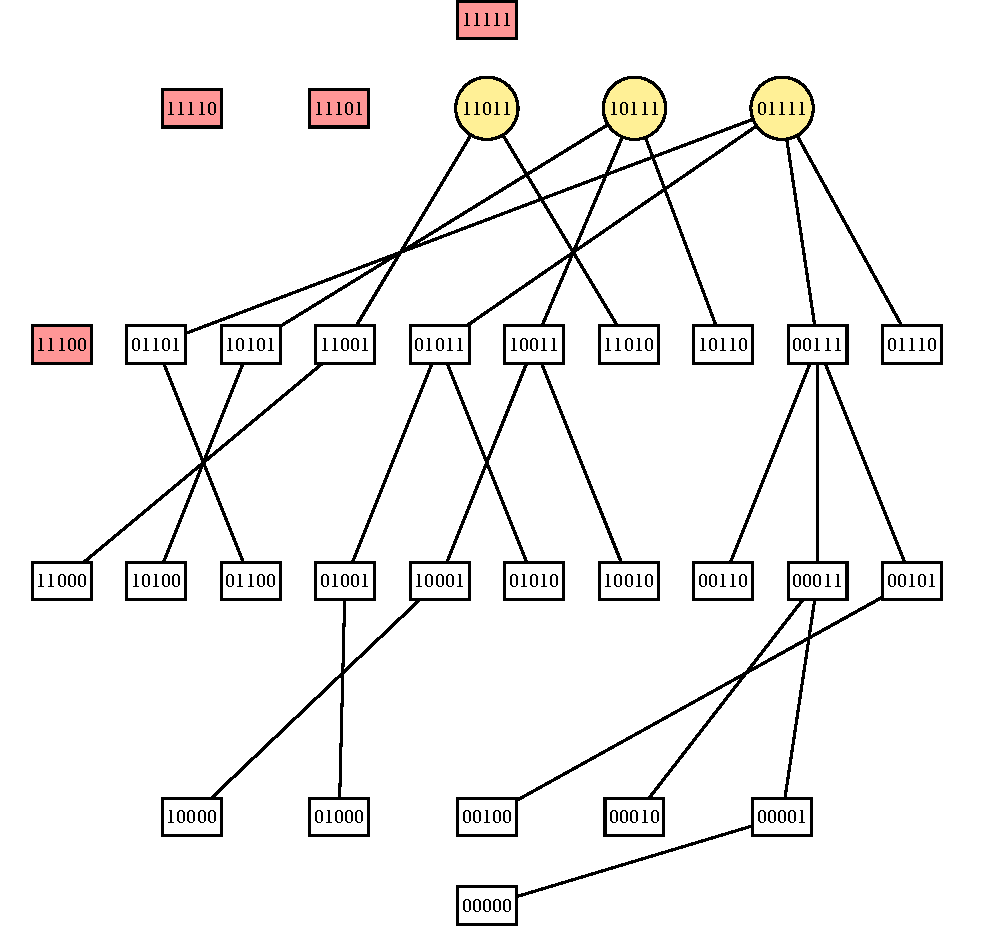
\includegraphics[clip=true]{pfs/pfs/forest/upper_tree.pdf}}
    \label{fig:ubb:tree} }
  \end{tabular}
  \end{figure}  
\end{frame}

\begin{frame}{O algoritmo \algname{Poset-Forest-Search}}
Podemos resumir o funcionamento do \algname{PFS} aos seguintes passos:
\pause
\begin{itemize}
  \item{Escolher uma direção de percorrimento}
  \pause
  \item{Percorrer uma cadeia da floresta escolhida}
  \pause
  \item{Sempre que a condição de poda for verdadeira:}
  \pause
    \begin{itemize}
    \item{Podar a floresta de percorrimento}
    \pause
    \item{Atualizar a floresta dual}
    \pause
    \end{itemize}
\end{itemize}
\end{frame}


%----------------------------------------------------------------------
\section{Melhoramentos ao \algname{Poset-Forest-Search}}


\begin{frame}{Melhoramentos na implementação atual do \algname{PFS}}
  O algoritmo implementado por Marcelo possui pontos que podiam ser
  explorados para se ter melhor desempenho computacional.
\end{frame}


\begin{frame}{Mudanças na escolha de raízes}
A implementação de Marcelo escolhia \alert{arbitrariamente} como raiz de
percorrimento a primeira quando ordenadas lexicograficamente.
\vspace{2em}\\
\pause
Propomos duas estratégias de escolhas:
\begin{itemize}
  \item{escolha aleatória e uniforme entre raízes;}
  \pause
  \item{escolha da raiz com maior sub-árvore.}
\end{itemize}
\end{frame}


\begin{frame}{Resultados da mudança de escolha de raízes}
Chamamos a variação do \algname{PFS} que escolhe raízes de maneira 
aleatória e identicamente provável de \algname{PFS-RAND}.

\pause

\begin{figure}[ht]
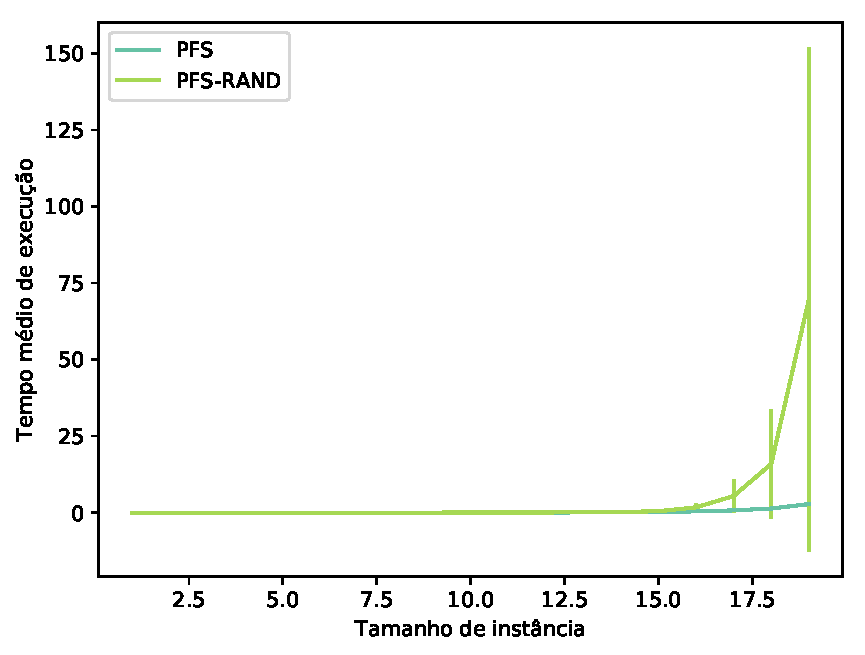
\includegraphics[clip=true, width=.5\textwidth]{pfs/pfs_rand_avg_time.pdf}
\end{figure}

\pause

A versão que escolhia a raiz com maior sub-árvore não teve bom 
desempenho.
\end{frame}


\begin{frame}{Melhoramentos na estrutura de armazenamento de raízes}
  Mudamos a implementação de Marcelo para usar diagramas de decisão
  binários ordenados (OBDDs).
  \pause
  \begin{figure}[]
  \centering 
  \begin{tabular}{c c}
    \subfigure {\scalebox{.5}{
     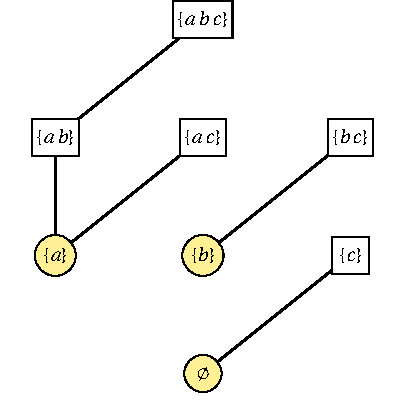
\includegraphics[clip=true]{pfs/obdd/lattice.pdf}}
     \label{fig:pfs:obdd:A} }
      & 
      \subfigure {\scalebox{.65}{
    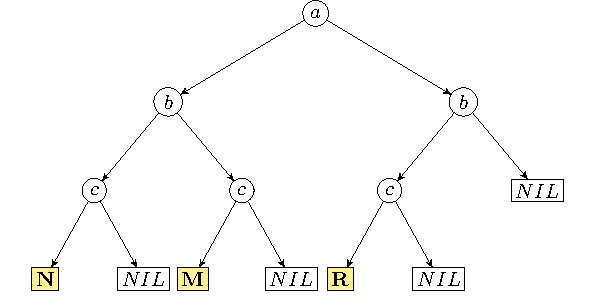
\includegraphics[clip=true]{pfs/obdd/obdd.pdf}}
    \label{fig:pfs:obdd:B} }
  \end{tabular}
  \end{figure}
\end{frame}


\begin{frame}{Resultados da mudança de estrutura para armazenamento de raízes}
Chamamos de \algname{OPFS} o algoritmo que usa OBDDs para armazenamento
de raízes.
\pause
\begin{figure}[ht]
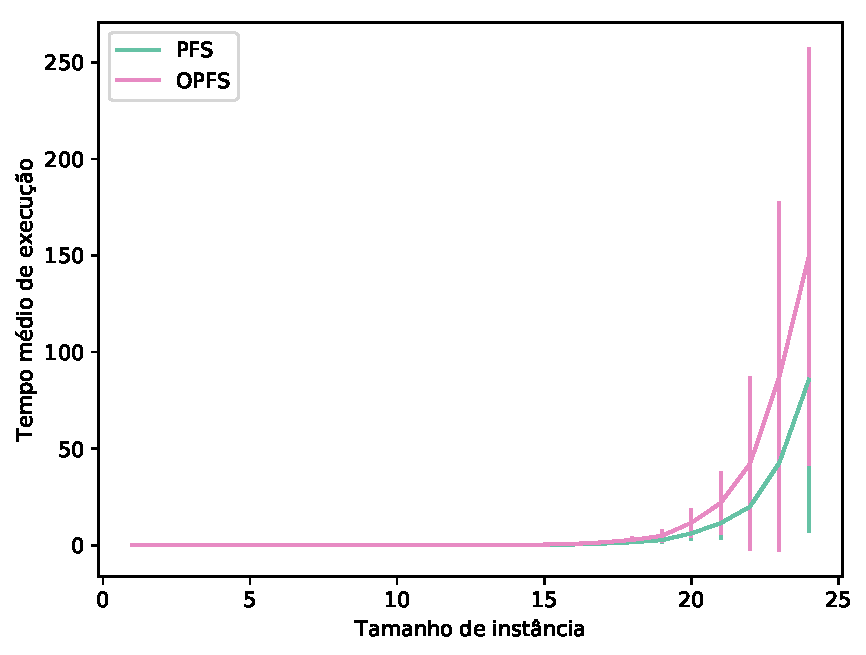
\includegraphics[clip=true, width=.7\textwidth]{pfs/opfs_avg_time.pdf}
\end{figure}
\end{frame}


\begin{frame}{Paralelização do \algname{PFS}}
Implementamos também uma versão paralela do algoritmo \algname{PFS}.
\vspace{1em}
\pause\\

Entretanto, a etapa de atualização da floresta dual é complicada e pode 
gerar condições de corrida, o que deixou a paralelização complicada.
\end{frame}

\begin{frame}{O algoritmo \algname{UBB-PFS}}
Este algoritmo é uma nova alternativa paralela que é dividida em duas
partes:
\vspace{1em}
\pause\\
\begin{itemize}
  \item{Percorrimento sequencial: idêntico ao \algname{UBB} deve criar
    sub-árvores no espaço enquanto faz uma ramificação do tipo
    busca em profundidade.}
  \pause
  \item{Solução em paralelo: cada sub-árvore gerada na etapa de 
    ramificação deve ser resolvida por uma chamada do \algname{PFS}.}
\end{itemize}
\end{frame}


\begin{frame}{Resultados do \algname{UBB-PFS}}
O \algname{UBB-PFS} foi mais rápido do que o \algname{PFS}.
\pause
\begin{figure}[ht]
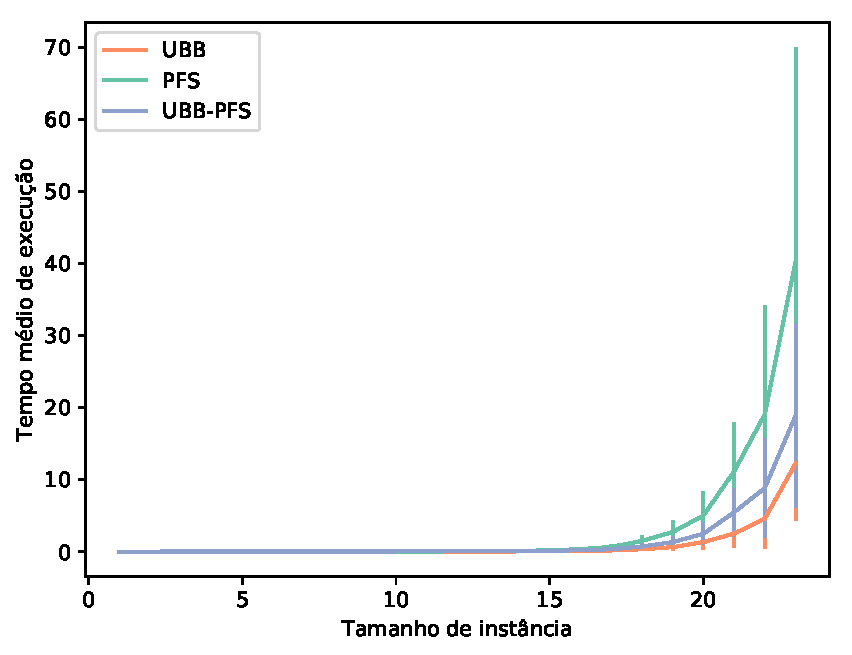
\includegraphics[clip=true, width=.7\textwidth]{pfs/ubb-pfs_avg_time.pdf}
\end{figure}
\end{frame}


\begin{frame}{Resultados do \algname{UBB-PFS}}
E computou menos a função custo do que o \algname{UBB}.
\begin{figure}[ht]
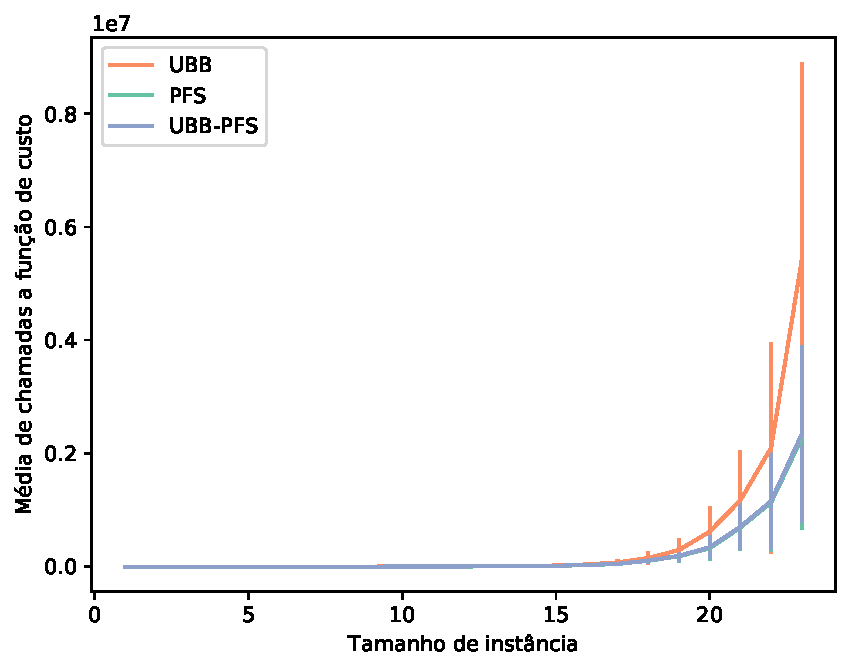
\includegraphics[clip=true, width=.7\textwidth]{pfs/ubb-pfs_avg_calls.pdf}
\end{figure}
\end{frame}


% ----------------------------------------------------------------------
\section{O algoritmo \algname{Parallel-U-Curve-Search}}

\begin{frame}{Ideia do \algname{Parallel-U-Curve-Search} (\algname{PUCS})}
    Um algoritmo de fácil paralelização e pouco entrelace de linhas
    de processamento, \pause e que também distribua o trabalho em partes
    de tamanho parecido.\pause \\
    \vspace{1em}
    Fazemos isso ao definir um particionamento do espaço.
\begin{figure}[!ht]
  \centering 
  \begin{tabular}{c c}
    \subfigure {\scalebox{0.23}{
    \includegraphics[clip=true]{pucs/partition/full_lattice.pdf}}}
    &
    \subfigure {\scalebox{0.23}{
    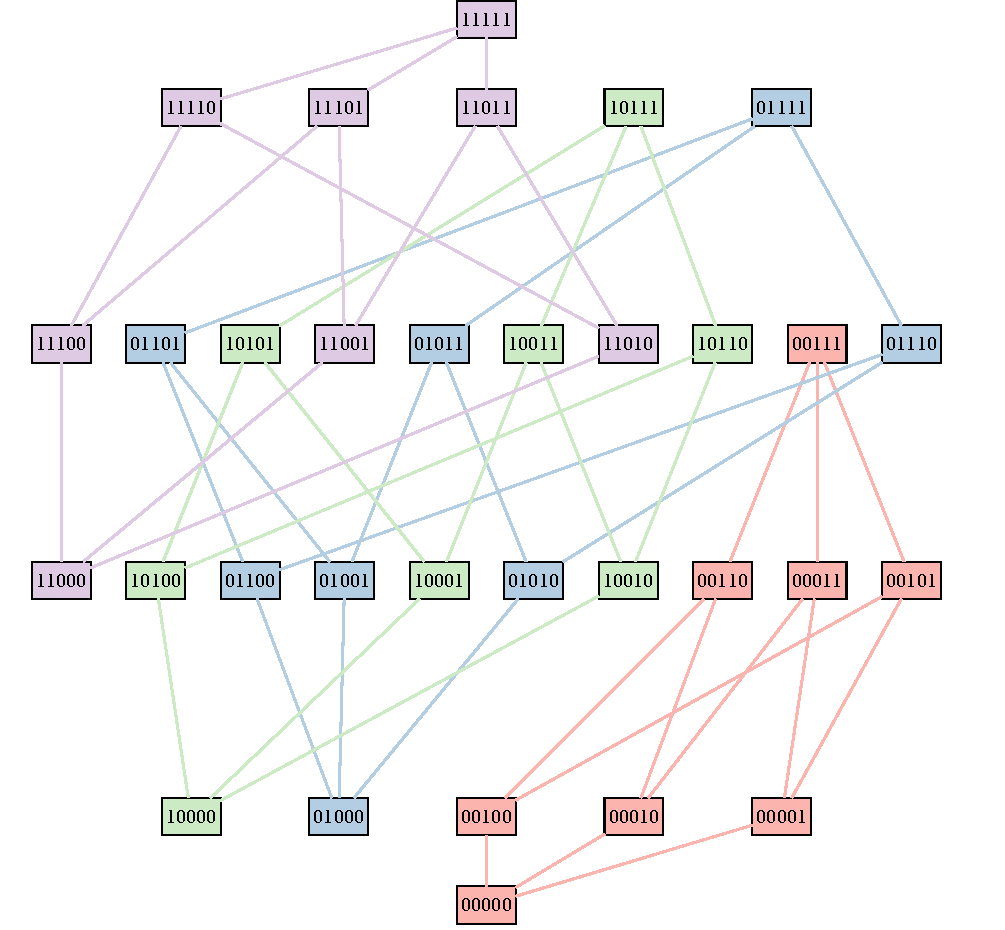
\includegraphics[clip=true]{pucs/partition/all_parts.pdf}}}\\
  \end{tabular}
\end{figure}
\end{frame}


\begin{frame}{Particionamento do espaço de busca}
Para particionar o espaço, escolhemos um conjunto arbitrário de 
variáveis $S'$. \pause

Agora, definimos a relação de equivalência para os conjuntos de 
características: \\
\begin{center}
$
\begin{aligned}
    X \sim Y \iff (X \cap S') = (Y \cap S')
\end{aligned}
$
\end{center}
\end{frame}

\begin{frame}{Estrutura recursiva do problema}
    Se representamos cada parte por um subconjunto de características de
    $S'$, então temos um reticulado Booleano de partes. Chamamos este
    reticulado de \alert{reticulado externo}.
    \vspace{1em}\\
    \pause
    Se representamos, cada nó de uma parte por um subconjunto de 
    características de $S - S'$, então temos um reticulado Booleano
    de nós de uma parte. Chamamos este reticulado de \alert{reticulado
    interno}.
\end{frame}

\begin{frame}{Estrutura recursiva do problema}
    \begin{figure}
    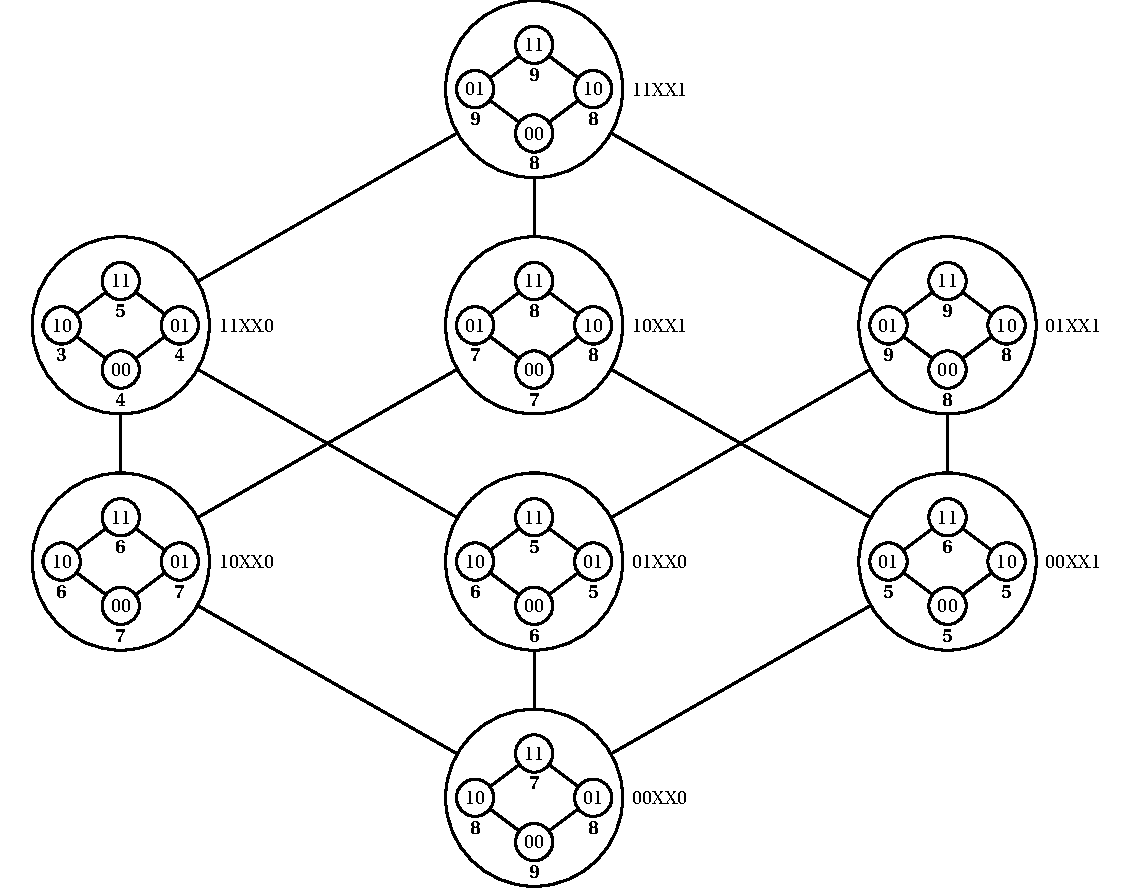
\includegraphics[clip=true, width=0.68\textwidth]{pucs/sample_run/A.pdf}
    \end{figure}
\end{frame}

\begin{frame}{Dinâmica}
    Podemos resumir a dinâmica deste algoritmo nos passos:
    \begin{itemize}
    \item{passeio aleatório no reticulado externo, com podas;}
    \item{solução de partes não podadas;}
    \item{união de respostas das partes.}
    \end{itemize}
\end{frame}


\begin{frame}{Simulação de execução}
    \begin{figure}[!ht]
    \begin{center}
    \begin{tabular}{l r}
    \centering
    \subfigure{
        \label{fig:pucs:example:lattice}
        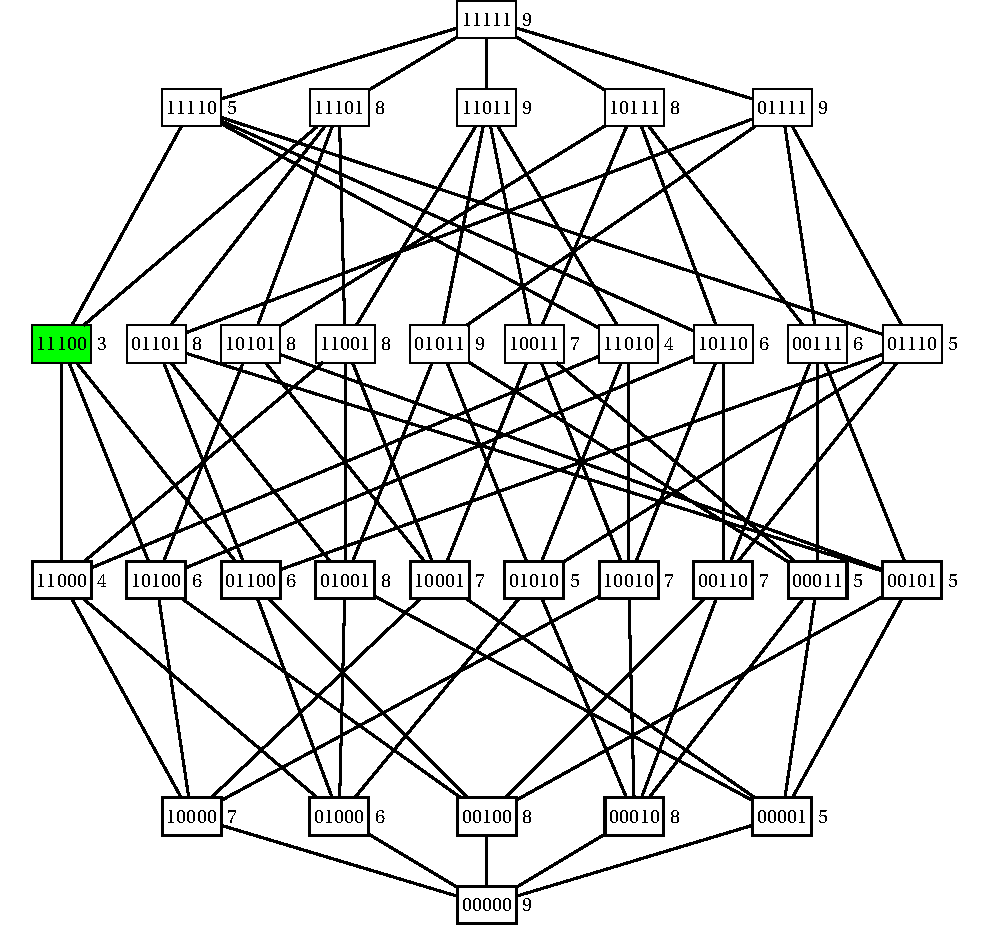
\includegraphics[clip=true, width=0.48\textwidth]{pucs/sample_run/Boolean_lattice.pdf}
    }
    &
    \subfigure{
        \label{fig:pucs:example:A}
        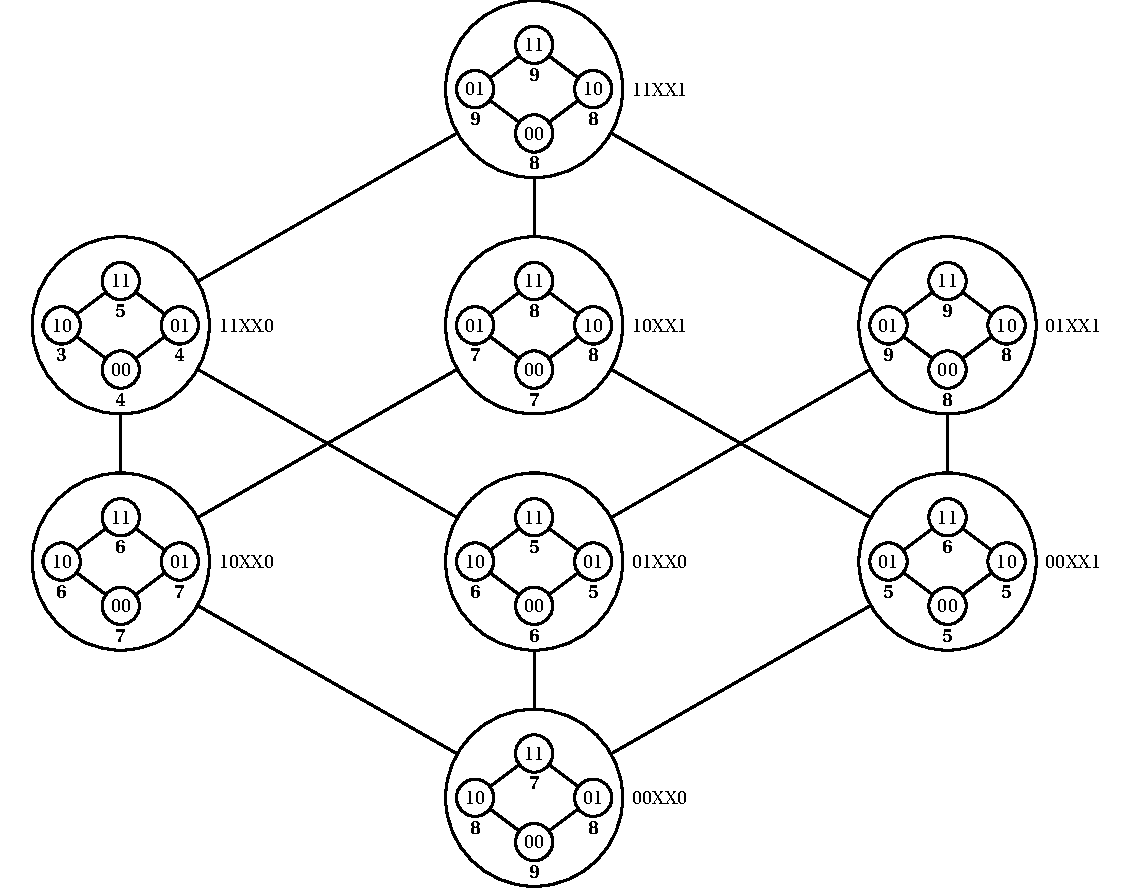
\includegraphics[clip=true, width=0.48\textwidth]{pucs/sample_run/A.pdf}
    }
    \end{tabular}   
    \end{center}
\end{figure}
\end{frame}

\begin{frame}{Simulação de execução}
    \begin{figure}[!ht]
    \begin{center}
    \begin{tabular}{l r}
    \centering
    \subfigure {
        \label{fig:pucs:example:B}
        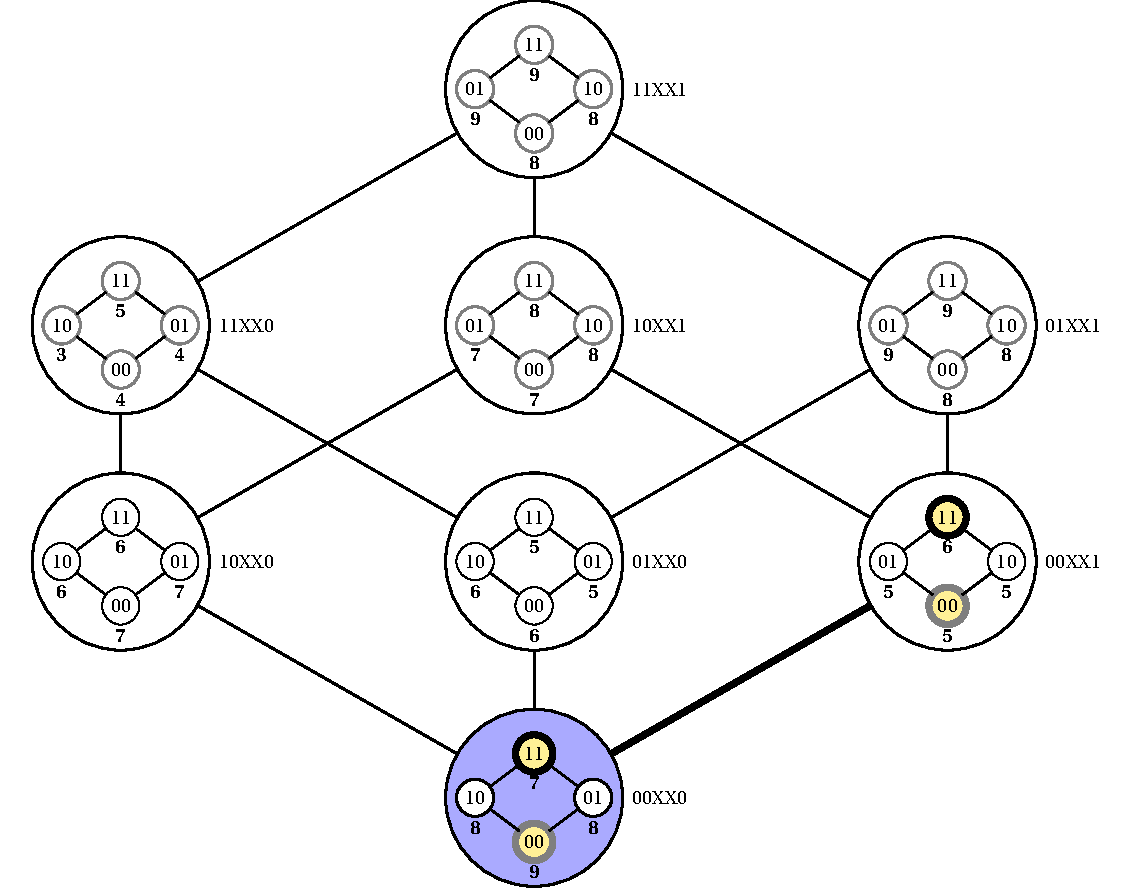
\includegraphics[ clip=true, width=0.4\textwidth]{pucs/sample_run/B.pdf}
    } \pause
    &
    \subfigure {
        \label{fig:pucs:example:C}
        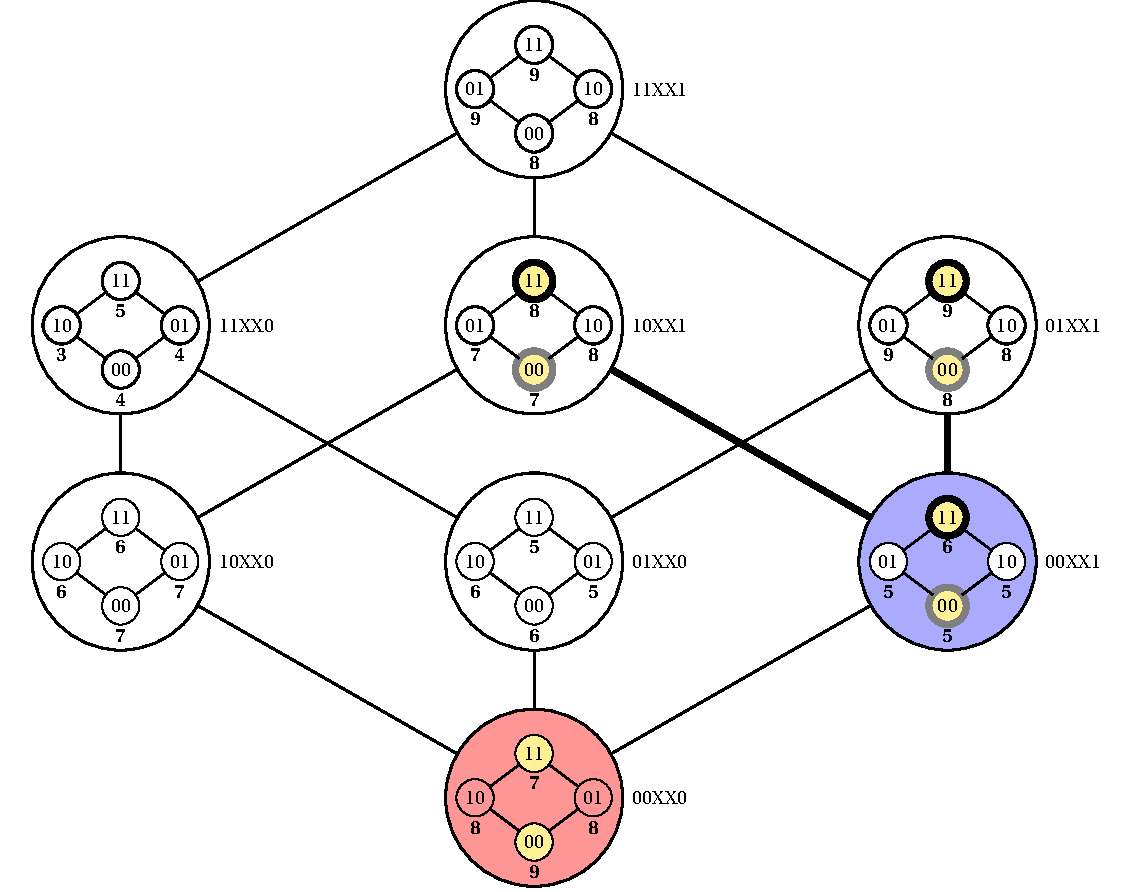
\includegraphics[clip=true, width=0.4\textwidth]{pucs/sample_run/C.pdf}
    }
    \vspace{1em}\pause\\ 
    \subfigure {
        \label{fig:pucs:example:D}
        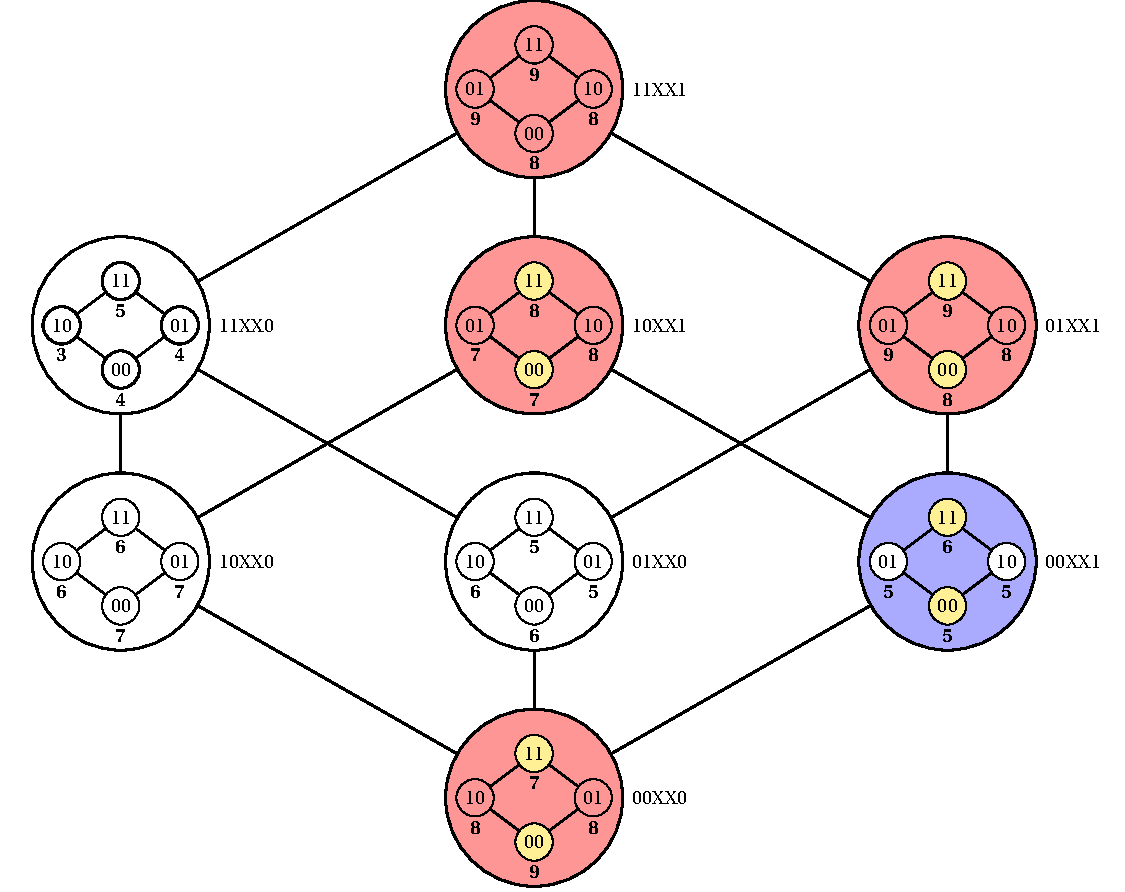
\includegraphics[ clip=true, width=0.4\textwidth]{pucs/sample_run/D.pdf}
    } \pause
    &
    \subfigure {
        \label{fig:pucs:example:E}
        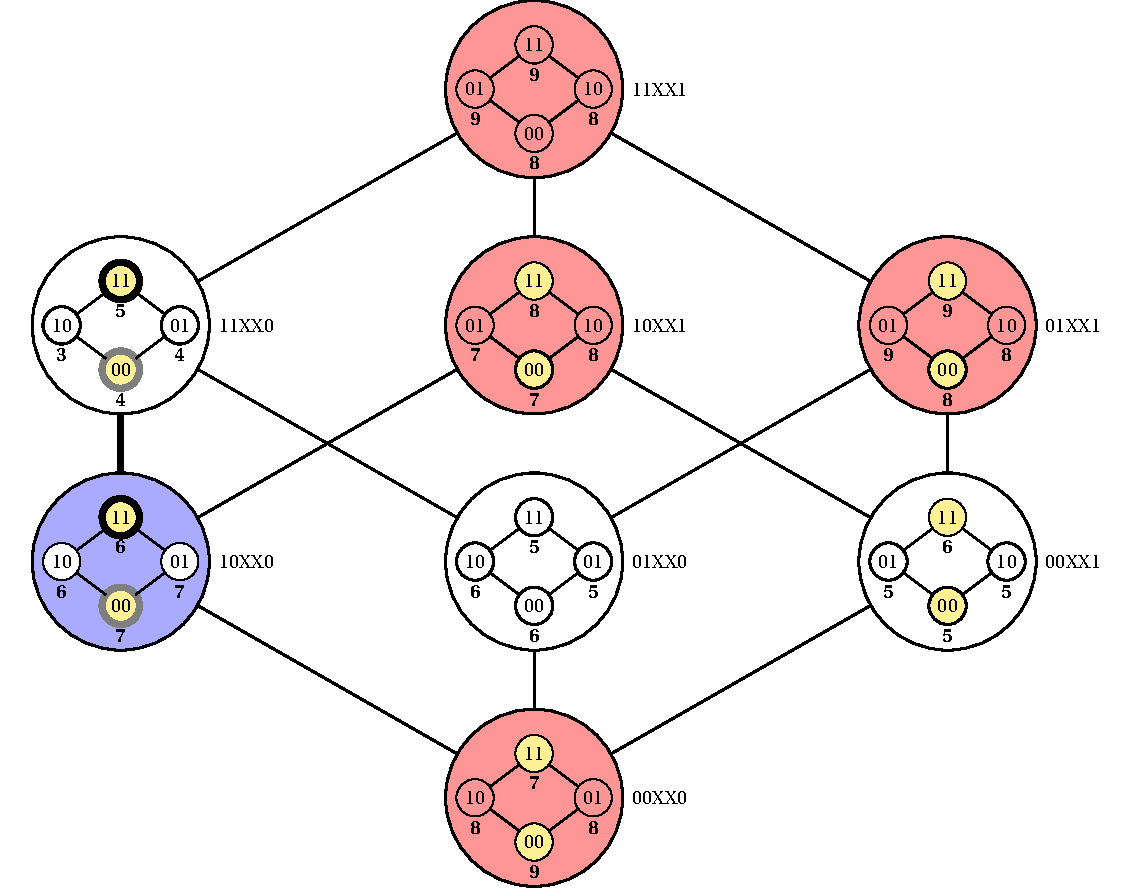
\includegraphics[clip=true, width=0.4\textwidth]{pucs/sample_run/E.pdf}
    }
    \end{tabular}   
    \end{center}
\end{figure}
\end{frame}


\begin{frame}{Simulação de execução}
\begin{figure}[]
    \begin{center}
    \begin{tabular}{l r}
    \centering
    \subfigure {
        \label{fig:pucs:example:F}
        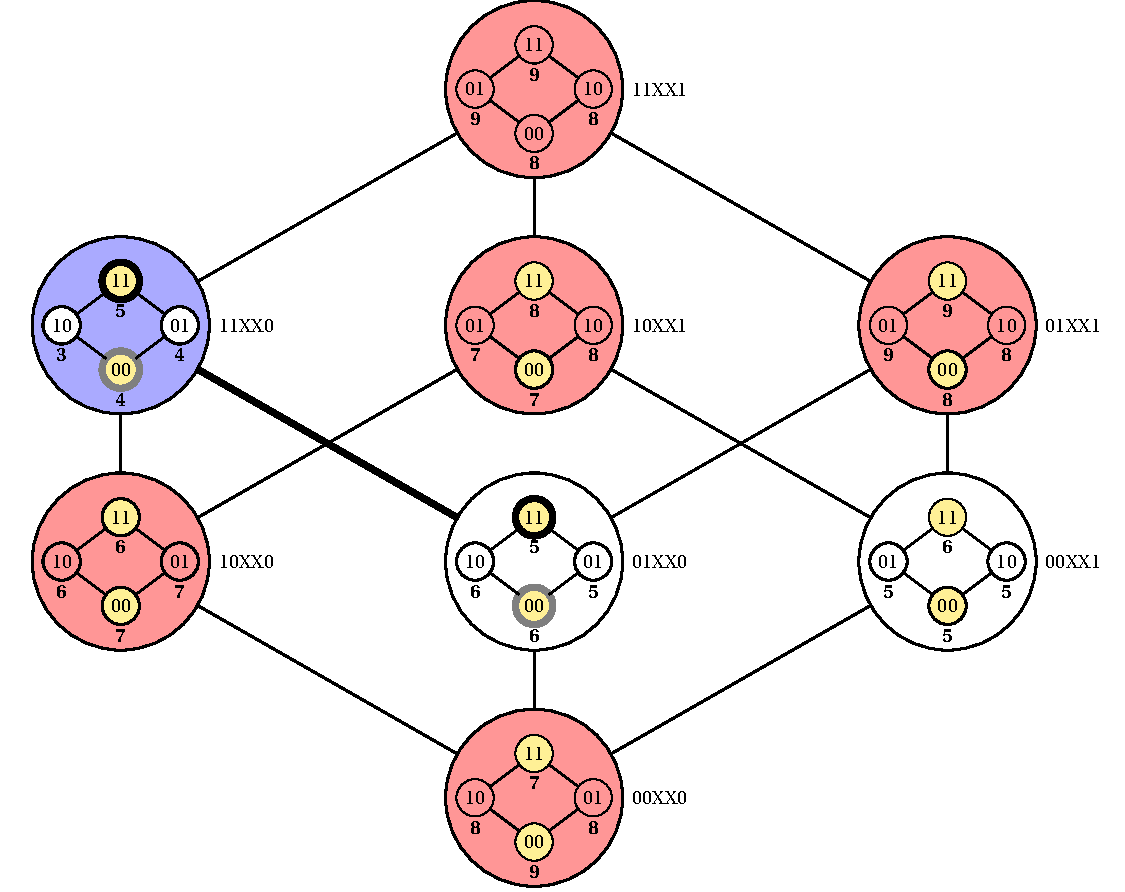
\includegraphics[ clip=true, width=0.4\textwidth]{pucs/sample_run/F.pdf}
    } \pause
    &
    \subfigure {
        \label{fig:pucs:example:G}
        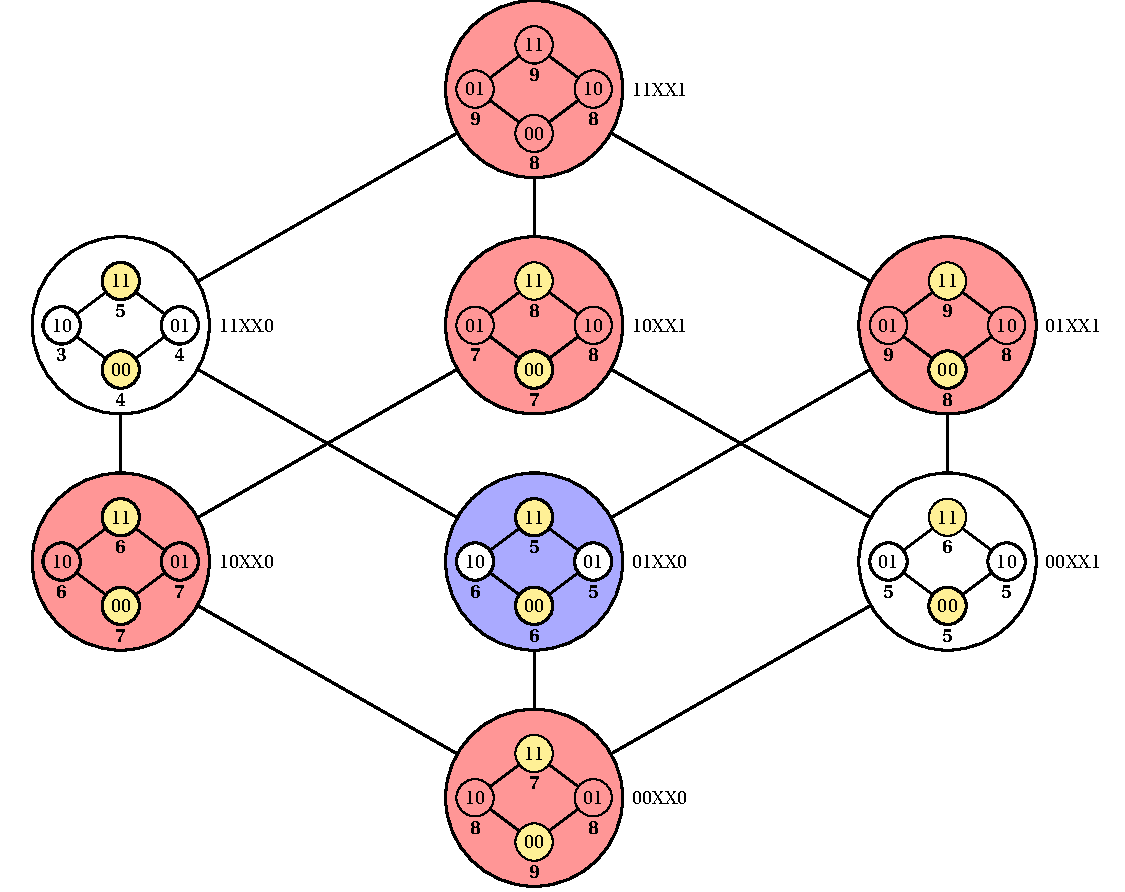
\includegraphics[clip=true, width=0.4\textwidth]{pucs/sample_run/G.pdf}
    }
    \vspace{1em}\pause\\
    \subfigure {
        \label{fig:pucs:example:H}
        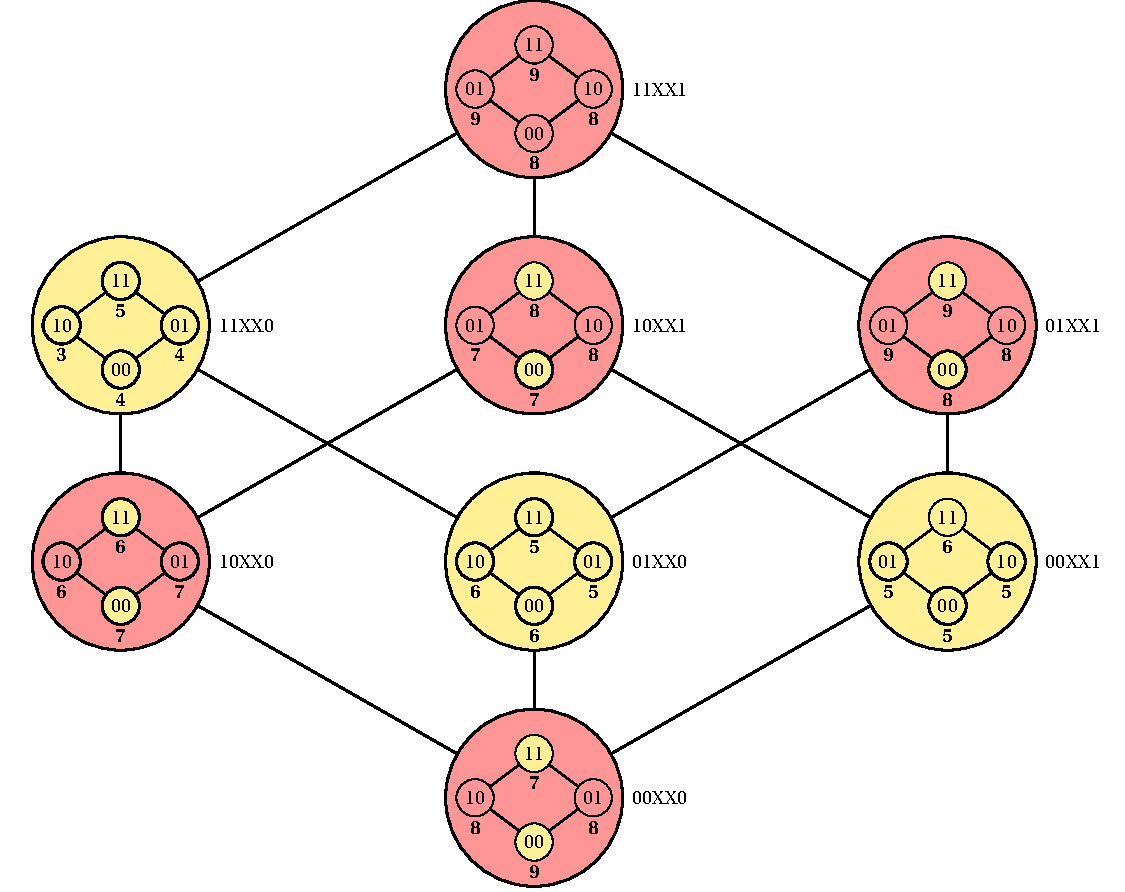
\includegraphics[ clip=true, width=0.4\textwidth]{pucs/sample_run/H.pdf}
    } \pause
    &
    \subfigure {
        \label{fig:pucs:example:I}
        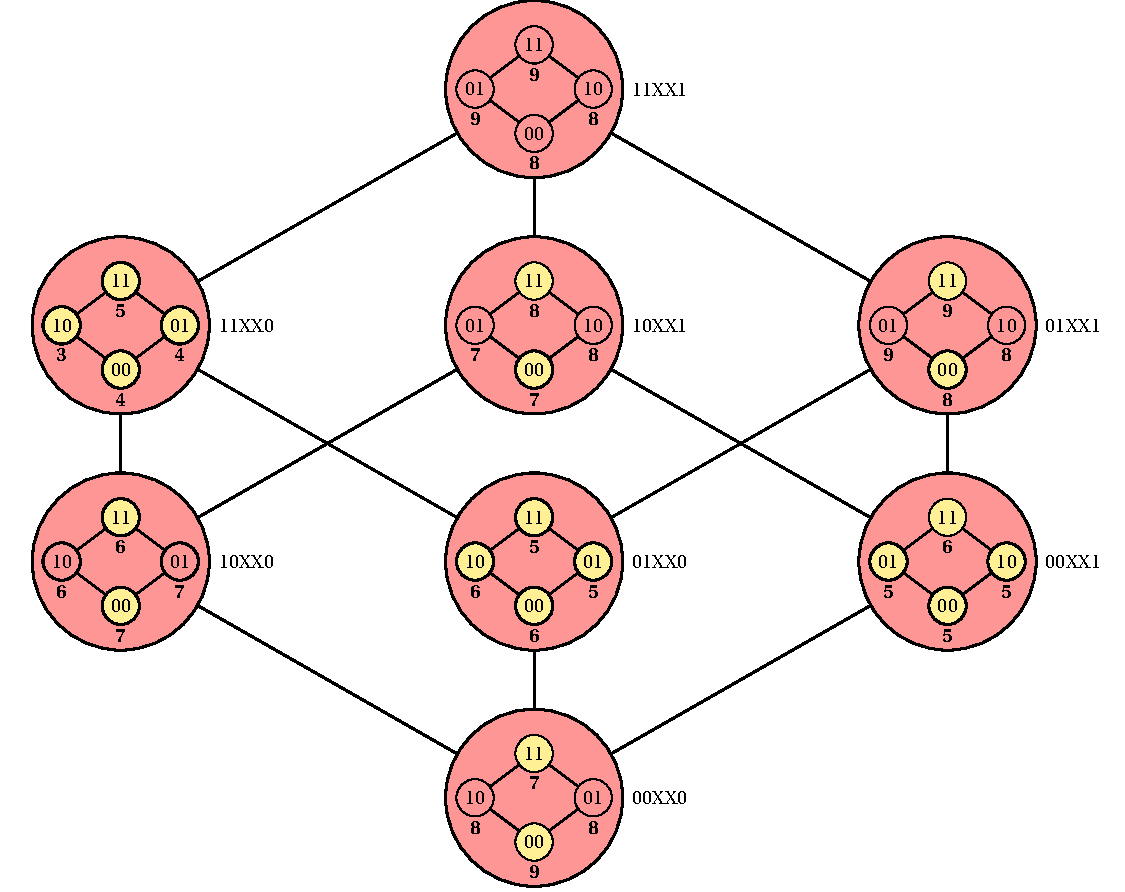
\includegraphics[clip=true, width=0.4\textwidth]{pucs/sample_run/I.pdf}
    }
    \end{tabular}   
    \end{center}
\end{figure}
\end{frame}


\begin{frame}{Resultados do \algname{PUCS}}
    Em instâncias pequenas, usamos parâmetros que deixam o algoritmo 
    ótimo. O desempenho do \algname{PUCS} foi similar ao do 
    \algname{UBB-PFS}.
\end{frame}

\begin{frame}{Resultados do \algname{PUCS}}
Em experimentos sub-ótimos, comparamos o \algname{PUCS} com as 
heurísticas \algname{Sequential Forward Floating Search} 
(\algname{SFFS}) e \algname{Best-First Search} (\algname{BFS}).
\begin{figure}[!ht]
\begin{center}
\begin{tabular}{l r}
\centering
\subfigure {
    \label{fig:pucs:big:time}
    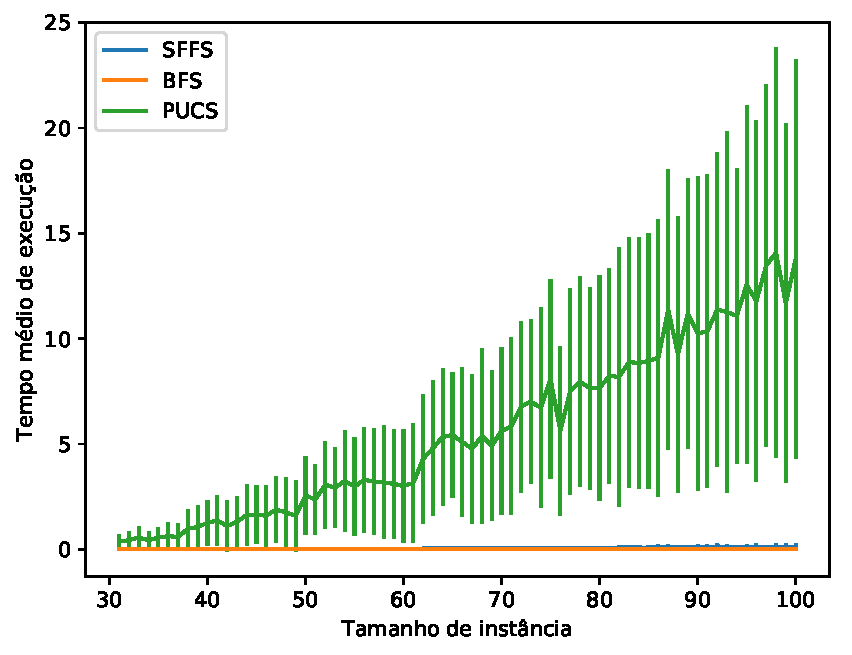
\includegraphics[clip=true, width=0.45\textwidth]{pucs/experiments/time_sffs_bfs_pucs.pdf}
}
&
\subfigure {
    \label{fig:pucs:big:correctness}
    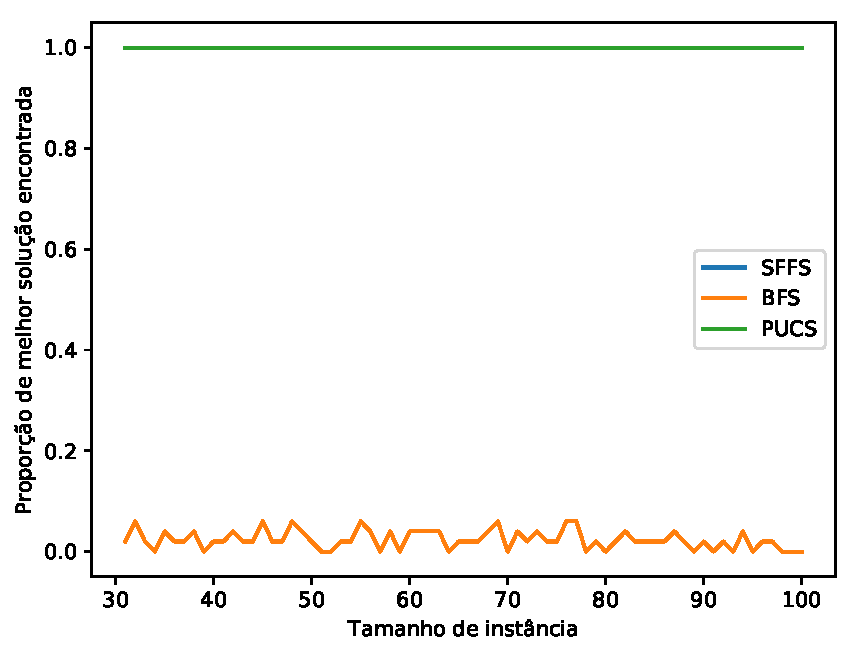
\includegraphics[clip=true, width=0.45\textwidth]{pucs/experiments/correctness_sffs_bfs_pucs.pdf}
}
\end{tabular}   
\end{center}
\end{figure}
\end{frame}

\section{Aplicações instâncias reais}

\begin{frame}{Seleção de características em seleção de modelos}
    Aplicamos seleção de características na construção de modelos
    de aprendizado para conjuntos de dados do UCI Machine Learning
    Repository.
\end{frame}

\begin{frame}{Modelos de aprendizado}
    Os modelos que utilizamos para o treinamento e classificação
    são do tipo Support Vector Machine.
    \begin{figure}
        \centering
        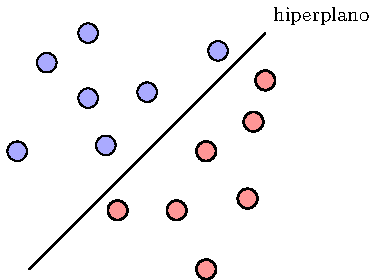
\includegraphics[clip=true, width=.5\textwidth]{svm/svm.pdf}
    \end{figure}
\end{frame}

\begin{frame}{Conjuntos de dados testados}
Fizemos o treinamento e validação de modelos de aprendizado nos 
seguintes conjuntos de dados: \pause
    \begin{itemize}
        \item{Iris} \pause
        \item{Wine} \pause
        \item{Thoracic Surgery} \pause
        \item{Zoo} \pause
        \item{Breast Cancer} \pause
        \item{Lung Cancer} \pause
        \item{Promoters} \pause
    \end{itemize}
\end{frame}


\begin{frame}{Validação cruzada}
Para avaliar a seleção de características fizemos a validação cruzada
de modelos com todas características e a de modelos apenas com 
características selecionadas.
\end{frame}

\begin{frame}{Resultados}
    O número de características selecionadas é, de fato, menor do que
    o conjunto inteiro.\pause
    \begin{figure}
        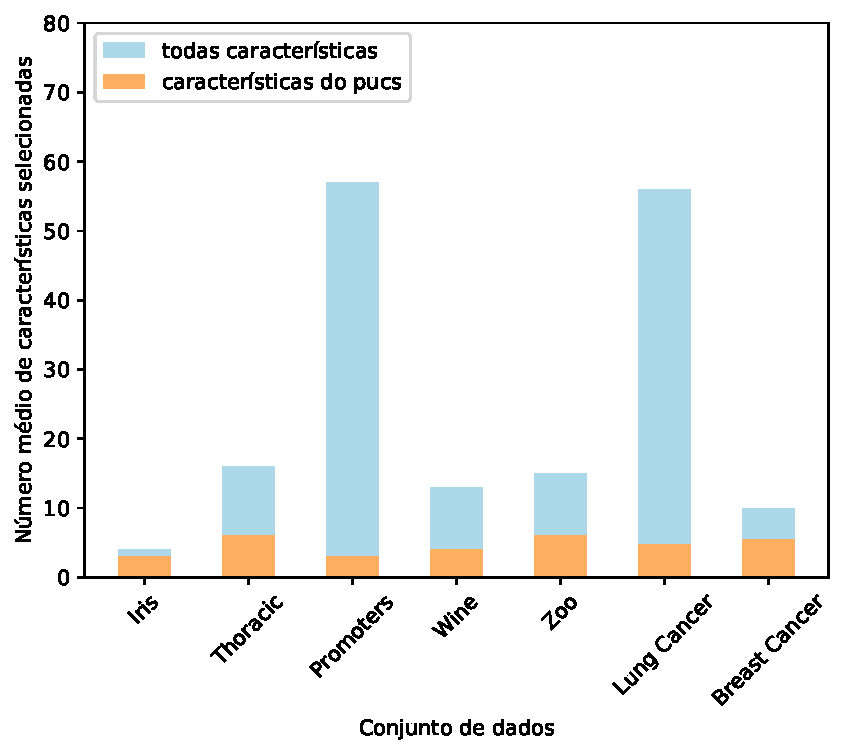
\includegraphics[clip=true, width=0.6\textwidth]{uci/avg_features.pdf}
    \end{figure}
\end{frame}

\begin{frame}{Resultados}
    Além disso, a qualidade dos modelos não é afetada. \pause
    \begin{figure}
        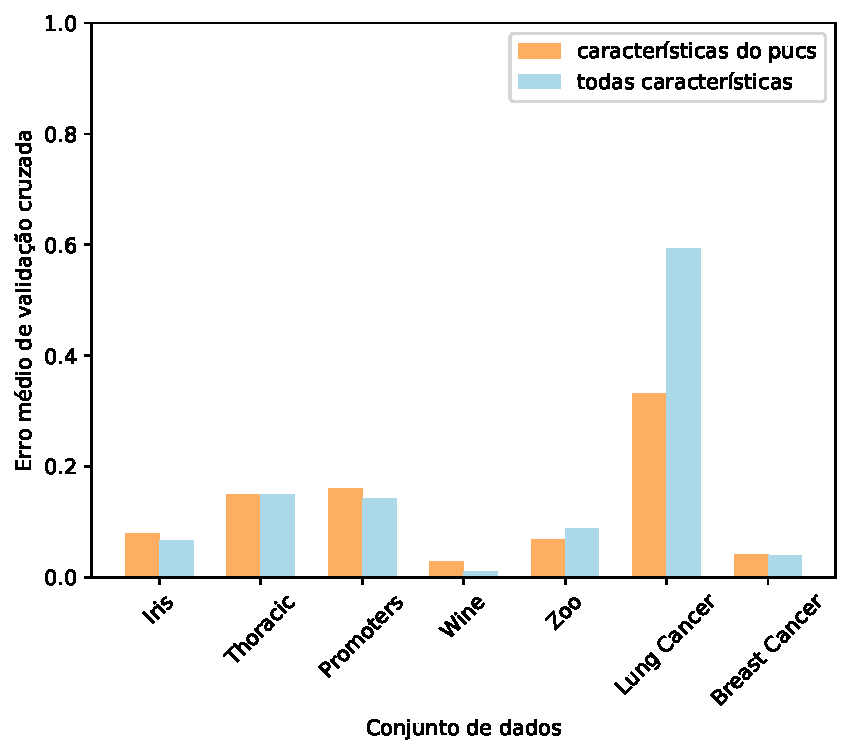
\includegraphics[clip=true, width=0.6\textwidth]{uci/svm_error.pdf}
    \end{figure}
\end{frame}

\section{Revisão}
\begin{frame}{Revisão dos resultados deste trabalho}
Ao longo deste trabalho apresentamos \pause
    \begin{itemize}
        \item{Modificações no \algname{PFS}.}
        \begin{itemize}
            \item{Escolha de raízes.}
            \item{Estrutura de dados para armazenamento de raízes.}
        \end{itemize} \pause
        \item{Uma paralelização do \algname{PFS}.} \pause
        \item{O algoritmo \algname{UBB-PFS}.} \pause
        \item{O algoritmo \algname{PUCS}.} \pause
        \item{Testes com instâncias reais.} \pause
    \end{itemize}
\end{frame}
\end{document}


